\documentclass{article}

\usepackage{cancel}
\usepackage{tikz}
\usepackage{amsmath}
\usepackage{geometry}
\usepackage{graphicx}
\usepackage{amsfonts} 
\usepackage{verbatim}
\usepackage{mathrsfs}  
\usepackage{lmodern}
\usepackage{braket}
\usepackage{circuitikz}
\usepackage{steinmetz}


\usetikzlibrary{quotes,angles,decorations.pathmorphing,shapes.geometric}
\tikzset{snake it/.style={decorate, decoration=snake},
         block/.style = {draw, fill=white, very thick, rectangle, minimum height=1cm, minimum width=2cm},
         sum/.style= {draw, fill=white, very thick, circle, node distance=1cm},
         triangle/.style= {draw, fill=white, very thick, isosceles triangle, minimum height=2cm, minimum width=1cm}}  
\numberwithin{equation}{subsection}
\graphicspath{ {./Immagini/} }

\renewcommand{\contentsname}{Indice}

%   To Do List:
%
%
% V Introduzione;
% V Modellistica;
%   Ingressi di Tipo Sinusoidale;
%   Controllori Digitali;
%   Esonero, potenzialmente;
%   Finire Con Equazioni Differenziali e Laplace;
% V Sostituire Immagini Screenate da Simulink con Blocchi Fatti in Tikz(https://latexdraw.com/block-diagram-in-latex-step-by-step-tikz-tutorial)e
%                                                                       (https://tex.stackexchange.com/questions/175969/block-diagrams-using-tikz);
%   Rotore DC grafico in CiruiTikz;





\title{Fondamenti di Automatica}
\author{}
\date{}

\begin{document}

\maketitle

\clearpage

\tableofcontents

\clearpage

\section{Introduzione}

L'atumotica è la scienza che si occupa dell'analisi del controllo di sistemi dinamici in quattro passaggi:
\begin{itemize}
    \item Modellazione: Rappresentazione matematica basata sulla fisica del sistema;
    \item Studio delle Soluzioni: Le solusioni possono essere ottenute analiticamente, in forma chiusa, o tramite simulazioni del dato sistema;
    \item Esplorazione: Ricerca di relazioni tra struttura e comportamento del sistema ed approfondimento di quest'ultimo;
    \item Modifica e Controllo: RIcerca dei metodi per cambiare il comportamento del sistema.
\end{itemize}
Un sistema (dal greco s\'{y}n + hist\'{a}nai) viene definito come un insieme di oggetti connessi, indipendenti, che operano insieme.
La decomposizione funzionale di un sistema, è un tipo di scomposizione che esprime le relazioni causa-effetto necessarie per comprendere il 
funzionamento del sistema e per poter intervenire su di esso. 
Questa scomposizione è formata da vari blocchi funzionali, vengono rappresentati come degli oggetti aventi due ingressi e due uscite, e dei parametri 
interni che ne descrivono il legame, un singolo blocco funzionale può quindi essere analizzato come un sistema a sé. In un blocco funzionale possono 
entrare degli ingressi scelti arbitrariamente $u(t)$, di cui è possibile 
controllare li comportamento, e disturbi $z(t)$, ovvero errori che agiscono indipendentemente sul blocco, non controllabili. Da un blocco funzionale 
escono l'uscita $y(t)$, funzione rispetto alle entrate scelte, ed una catena di misura, usata per anlizzare uno o tutti i parametri di $y(t)$. 
Il comportamento di un singolo blocco viene rappresentato come dei parametri $\sum$ costanti, che rappresentano il comportamento fisico del blocco, 
e ne descrivono le sue uscite rispetto all'entrate date. 

\begin{center}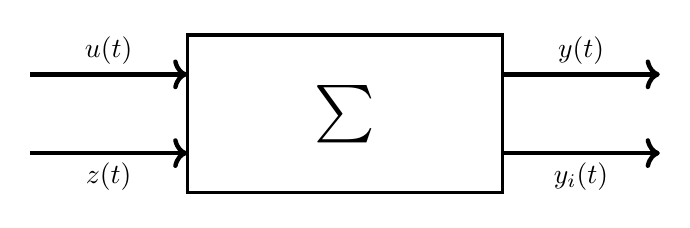
\begin{tikzpicture}[scale=2]

    \node[rectangle, draw, very thick, 
    minimum width = 4cm, 
    minimum height = 2cm] (r) at (0,0){\huge $\sum$};

    \draw[->,ultra thick](-2,0.25)--(-1,0.25);
    \node[above]at(-1.5,0.25){$u(t)$};

    \draw[->,ultra thick](-2,-0.25)--(-1,-0.25);
    \node[below]at(-1.5,-0.25){$z(t)$};

    \draw[->,ultra thick](1,0.25)--(2,0.25);
    \node[above]at(1.5,0.25){$y(t)$};

    \draw[->,ultra thick](1,-0.25)--(2,-0.25);
    \node[below]at(1.5,-0.25){$y_i(t)$};

\end{tikzpicture}\end{center}

Viene definito sistema isolato, un sistema in cui le uscite dipendono solo dagli ingressi attuali $\sum:y=f(u)$.

\begin{center}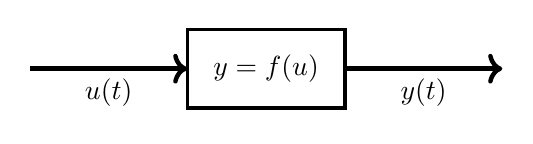
\begin{tikzpicture}[scale=2]
    \node[rectangle, draw, very thick, minimum width=2cm, minimum height=1cm](r)at(0,0){$y=f(u)$};

    \draw[->,ultra thick](-1.5,0)--(-0.5,0);
    \node[below]at(-1,0){$u(t)$};

    \draw[<-,ultra thick](1.5,0)--(0.5,0);
    \node[below]at(1,0){$y(t)$};

\end{tikzpicture}\end{center}

Viene definito sistema dinamico, un sistema le cui uscite dipendono dagli ingressi attuali e dagli ingressi passati del sistema 
$\sum:g(y^{(0)},...,y^{(n)},u^{(0)},...,u^{(m)})=0$.

\begin{center}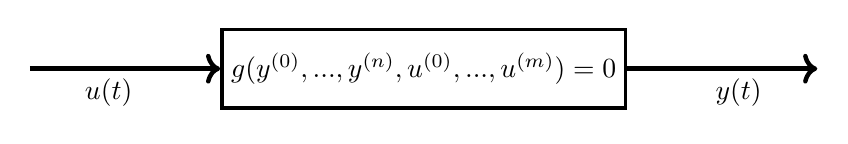
\begin{tikzpicture}[scale=2]
    \node[rectangle, draw, very thick, minimum width=2cm, minimum height=1cm](r)at(0,0){$g(y^{(0)},...,y^{(n)},u^{(0)},...,u^{(m)})=0$};

    \draw[->,ultra thick](-2.5,0)--(r.west);
    \node[below]at(-2,0){$u(t)$};

    \draw[<-,ultra thick](2.5,0)--(r.east);
    \node[below]at(2,0){$y(t)$};

\end{tikzpicture}\end{center}

Viene definito stato del sistema $\vec{x}(t)$, un vettore di $n$ variabili dipendenti dal tempo, tale che la conoscenza del suo valore 
allo stato $\vec{x}(t=0)$, e l'andamento dell'ingresso da $t=0$ in poi è sufficiente a determinare univocamente da $t=0$ in poi l'andamento di tutte le 
variabili dipendenti. 
In generale dato lo stato completo di un sistma in un istante di tempo $\vec{x}(t_0)$, è possible determinarne l'evoluzione futura, ovvero 
$\vec{x}(t>t_0)$. 

\clearpage

\section{Equazioni Differenziali}

\subsection{Introduzione alle Equazioni Differenziali}

\subsection{Equazioni Differenziali Ordinarie}

\subsection{Problema di Cauchy}

\subsection{Equazione Lineare di Primo Ordine}

\subsection{Equazione di Grado Superiore al Primo}

\subsubsection{Metodo Geometrico}

\subsubsection{Metodo Algebrico}

\clearpage

\section{Trasformata di Laplace}

\subsection{Trasformate Notevoli}

\subsection{Trasformata di un'Equazione Differenziale di Ordine Superiore al Primo}

\subsection{Stabilità di un Sistema}

\subsection{Funzioni di Trasferimento}
Una funzione di trasferimento del tipo ingresso-uscita, per cui perde ogni informazione sullo stato del sistema.
Se due funzioni di trasferimento si trovano in serie, allora si possono sostituire da un'altra funzione di trasferimento data dal prodotto dalle due, 
in generale per un numero $n$ di funzioni di trasferimento in serie si può descrivere una funzione equivalente $G(s)=\prod_{i=1}^nG_i(s)$. 

\begin{center}
    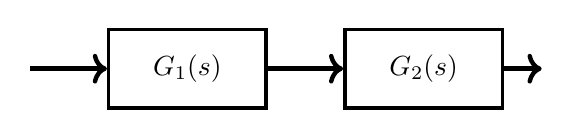
\begin{tikzpicture}[scale=2]
        \node[block, node distance=0cm](g1){$G_1(s)$};
        \node[block, right of=g1, node distance=3cm](g2){$G_2(s)$};
        \draw[->,ultra thick](g1.0)--(g2.180);
        \draw[->,ultra thick](-1,0)--(g1.180);
        \draw[->,ultra thick](g2.0)--(2.25,0);
    \end{tikzpicture}
\end{center}
\vspace{0.25cm}
\begin{center}
    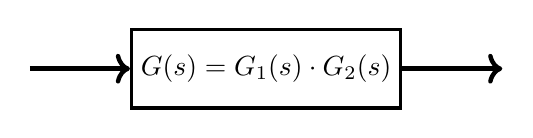
\begin{tikzpicture}[scale=2]
        \node[block, node distance=0cm](g){$G(s)=G_1(s)\cdot G_2(s)$};
        \draw[->,ultra thick](-1.5,0)--(g.180);
        \draw[->,ultra thick](g.0)--(1.5,0);
    \end{tikzpicture}
\end{center}

Date due funzioni di trasferimento in parallelo, potranno essere sostituite da un'altra funzinoe equivalente alla somma tra le due, in generale 
per $k$ funzioni di trasferimento in parallelo, potranno essere sostituite da un'altra funzione equivalente $G(s)=\sum_{i=1}^kG_i(s)$. 

\begin{center}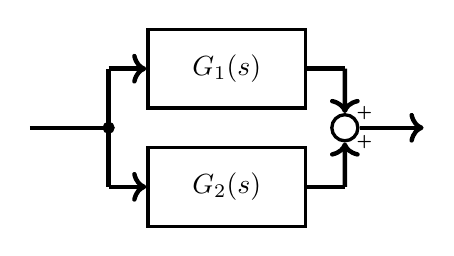
\begin{tikzpicture}[scale=2]
    \node[block, node distance=0cm](g1){$G_1(s)$};
    \node[block, below of=g1, node distance=1.5cm](g2){$G_2(s)$};
    \filldraw[black](-0.75,-0.375)circle(1pt)coordinate(split);
    \node[sum, right of=split, node distance=3cm](sum){};
    \draw[-,ultra thick](-1.25,-0.375)--(-0.75,-0.375);
    \draw[-,ultra thick](split)--(-0.75,0);
    \draw[-,ultra thick](split)--(-0.75,-0.75);
    \draw[->,ultra thick](-0.75,0)--(g1.180);
    \draw[->,ultra thick](-0.75,-0.75)--(g2.180);
    \draw[-,ultra thick](g1.0)--(0.75,0);
    \draw[-,ultra thick](g2.0)--(0.75,-0.75);
    \draw[->,ultra thick](0.75,0)--(sum.90)node[right]{$\scriptscriptstyle\boldsymbol{+}$};
    \draw[->,ultra thick](0.75,-0.75)--(sum.270)node[right]{$\scriptscriptstyle\boldsymbol{+}$};
    \draw[->,ultra thick](sum.0)--(1.25,-0.375);
\end{tikzpicture}\end{center}
\vspace{0.25cm}
\begin{center}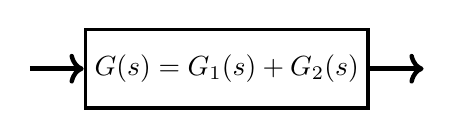
\begin{tikzpicture}[scale=2]
    \node[block](g){$G(s)=G_1(s)+G_2(s)$};
    \draw[->,ultra thick](-1.25,0)--(g.180);
    \draw[<-,ultra thick](1.25,0)--(g.0);
\end{tikzpicture}\end{center}

La funzione di trasferimento complessiva di un sistema presenta tutte le dinamiche di quel sistema, ovvero non viene persa l'informazione sulle 
dinamiche manipolando le funzioni di trasferimento. 
Per spostare una funzione di trasferimendo sulla catena bisogna opportunamente dividere e moltiplicare per tale funzione su tutte le altre 
ramificazioni per mantenere invariata l'entrata $U(s)$ su quella catena. 

\begin{center}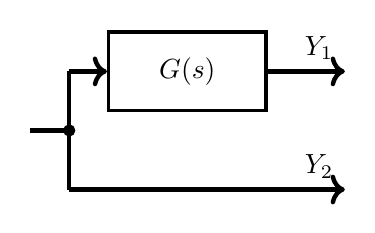
\begin{tikzpicture}[scale=2]
    \node[block](g){$G(s)$};
    \draw[-,ultra thick](-1,-0.375)--(-0.75,-0.375);
    \filldraw[black](-0.75,-0.375)circle(1pt);
    \draw[-,ultra thick](-0.75,-0.375)--(-0.75,0);
    \draw[->,ultra thick](-0.75,0)--(g.180);
    \draw[->,ultra thick](g.0)--(1,0)node[above left]{$Y_1$};
    \draw[-,ultra thick](-0.75,-0.375)--(-0.75,-0.75);
    \draw[->,ultra thick](-0.75,-0.75)--(1,-0.75)node[above left]{$Y_2$};
\end{tikzpicture}\end{center}
\vspace{0.25cm}
\begin{center}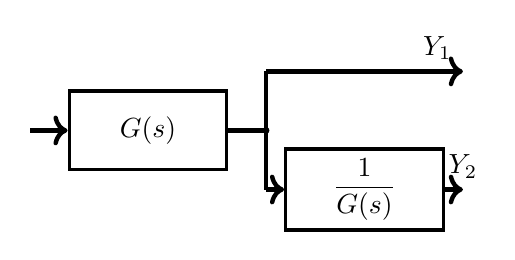
\begin{tikzpicture}
    \node[block](g){$\displaystyle\frac{1}{G(s)}$};
    \draw[-,ultra thick](-1.5,0.75)--(-1.25,0.75);
    \filldraw[black](-1.25,0.75)circle(1pt);
    \coordinate(o)at(-1.25,0.75);
    \draw[-,ultra thick](-1.25,0.75)--(-1.25,0);
    \draw[->,ultra thick](-1.25,0)--(g.180);
    \draw[->,ultra thick](g.0)--(1.25,0)node[above]{$Y_2$};
    \draw[-,ultra thick](-1.25,0.75)--(-1.25,1.5);
    \draw[->,ultra thick](-1.25,1.5)--(1.25,1.5)node[above left]{$Y_1$}; 
    \node[block, left of=o,node distance=1.5cm](g2){$G(s)$};
    \draw[-,ultra thick](g2.0)--(o);
    \draw[<-,ultra thick](g2.180)--(-4.25,0.75);
\end{tikzpicture}\end{center}

Viene definito processo di un sistema l'insieme coordinato di trasformazioni, trasmissione di energia, materiali e informazioni finalizzato ad un 
obiettivo, viene indicato con la funzione $P(s)$. 

Viene definito sistema a controreazione o retroreazione o feedback un sistema in cui l'uscita passata agisce sull'entrata futura. Si vuole calcolare 
una funzione di trasferimento equivalente:
\begin{equation}
    Y(s)=U(s)\cdot W(s)\Rightarrow W(s)=\displaystyle\frac{Y(s)}{U(s)}
\end{equation}    
Per trovarla si analizzano le varie entrate ed uscite del sistema. Quando si analizza una certa 
entrate o uscita, tutte le altre vengono consdierate nulle:
\begin{gather}
    \begin{cases}
        Y=eG\\
        e=U-HY
    \end{cases}\\
    \displaystyle\frac{Y}{G}=U-HY\\
    Y(1+GH)=UG\\
    \displaystyle\frac{Y}{U}=\frac{G}{1+GH}=W
\end{gather}
Viene definita la funzione del ciclo aperto, uguale al prodotto di ugni funzione di trasferimento lungo l'anello:
\begin{equation}
    F(s)=\prod_{i=1}^nG_i(s)
\end{equation}
Per cui la funzione di trasferimento del sistema a controreazione o funzione a ciclo chiuso può essere esrpessa come il rapporto tra la funzione di 
trasferimento a catena diretta, 
ovvere la funzione di trasferimento equivalente a tutte le funzioni di trasferimento tra l'ingresso $U$ all'uscita $Y$ senza passare per l'anello, e la 
somma tra $1$ e la funzione a ciclo aperto, con segno negativo se è presente un numero pari di cambi di segno, altrimenti positivo. 
\begin{equation}
    W(s)=\displaystyle\frac{G(s)}{1\pm F(s)}
\end{equation}

\begin{center}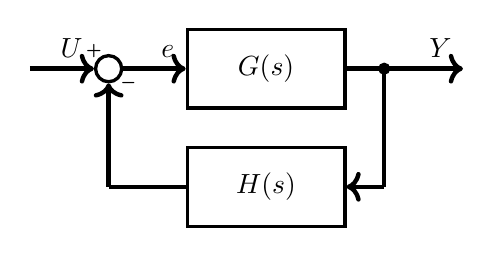
\begin{tikzpicture}[scale=2]
    \node[sum](sum)at(-1,0){};
    \draw[->,ultra thick](-1.5,0)--(sum.180)node[above left]{$U$}node[above]{$\scriptscriptstyle\boldsymbol{+}$};
    \node[block, right of=sum, node distance=2cm](g){$G(s)$};
    \draw[->,ultra thick](sum.0)--(g.180)node[above left]{$e$};
    \draw[-,ultra thick](g.0)--(0.75,0);
    \filldraw[black](0.75,0)circle(1pt);
    \draw[->,ultra thick](0.75,0)--(1.25,0)node[above left]{$Y$};
    \draw[-,ultra thick](0.75,-0.75)--(0.75,0);
    \node[block, below of=g, node distance=1.5cm](h){$H(s)$};
    \draw[->,ultra thick](0.75,-0.75)--(h.0);
    \draw[-,ultra thick](h.180)--(-1,-0.75);
    \draw[->,ultra thick](-1,-0.75)--(sum.270)node[right]{$\scriptscriptstyle\boldsymbol{-}$};
\end{tikzpicture}\end{center}

Se invece fosse presente un errore sulla catena diretta, allora per trovare la funzione a ciclo chiuso del disturbo, si considera:

\begin{gather}
    \begin{cases}
        e=-HY\\
        Y=eG+z
    \end{cases}\\
    Y=-GHY+z\\
    W_z=\displaystyle\frac{1}{1+GH}=\frac{1}{1+F}
\end{gather}

\begin{center}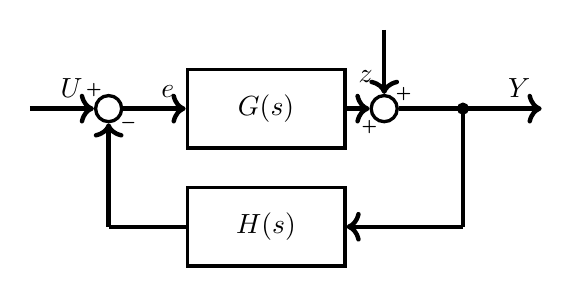
\begin{tikzpicture}[scale=2]
    \node[sum](sum)at(-1,0){};
    \node[sum](sum2)at(0.75,0){};
    \draw[->,ultra thick](-1.5,0)--(sum.180)node[above left]{$U$}node[above]{$\scriptscriptstyle\boldsymbol{+}$};
    \node[block, right of=sum, node distance=2cm](g){$G(s)$};
    \draw[->,ultra thick](sum.0)--(g.180)node[above left]{$e$};
    \draw[->,ultra thick](g.0)--(sum2.180)node[below]{$\scriptscriptstyle\boldsymbol{+}$};
    \draw[-,ultra thick](sum2.0)--(1.25,0);
    \filldraw[black](1.25,0)circle(1pt);
    \draw[->,ultra thick](0.75,0.5)--(sum2.90)node[above left]{$z$}node[right]{$\scriptscriptstyle\boldsymbol{+}$};
    \draw[->,ultra thick](1.25,0)--(1.75,0)node[above left]{$Y$};
    \draw[-,ultra thick](1.25,-0.75)--(1.25,0);
    \node[block, below of=g, node distance=1.5cm](h){$H(s)$};
    \draw[->,ultra thick](1.25,-0.75)--(h.0);
    \draw[-,ultra thick](h.180)--(-1,-0.75);
    \draw[->,ultra thick](-1,-0.75)--(sum.270)node[right]{$\scriptscriptstyle\boldsymbol{-}$};
\end{tikzpicture}\end{center}

Ogni errore sulla catena di misura genererà un'errore in uscita.\\

In generale la funzione a ciclo chiuso di una qualsiasi entrata di un qualsiasi sistema a controreazione avrà un denominatore $Dem(s)=1\pm F(s)$, dove $F(s)$ è la funzione a 
ciclo aperto del sistema considerato. Avendo tutte le stesso denominatore, 
se una funzione a ciclo chiuso per due generiche entrate e uscite del sistema è stabile, allora tutte le funzioni a ciclo chiuso del sistema sono 
stabili, e tutti gli oggetti in entrata saranno stabili.  

\clearpage

\section{Modellistica}

Per controllare il comportamento di un sistema, dopo aver analizzato l'entrata necessaria per ottenere l'effetto desiderato, si può 
implementare un controllore $C(s)$, che dato un ingresso lo manipola per poi restituirlo al processo $P(s)$ che agirà in base all'entrata modificata. 


Si può ottenere tramite un ciclo a feeedback:

\begin{center}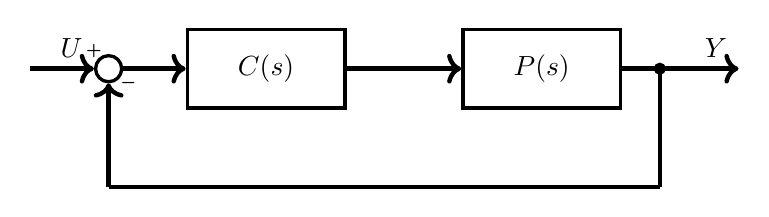
\begin{tikzpicture}[scale=2]
    \node[sum](sum)at(-1,0){};
    \draw[->,ultra thick](-1.5,0)--(sum.180)node[above left]{$U$}node[above]{$\scriptscriptstyle\boldsymbol{+}$};
    \node[block, right of=sum, node distance=2cm](c){$C(s)$};

    \draw[->,ultra thick](sum.0)--(c.180);
    \filldraw[black](2.5,0)circle(1pt);

    \draw[->,ultra thick](2.5,0)--(3,0)node[above left]{$Y$};
    \draw[-,ultra thick](2.5,-0.75)--(2.5,0);

    %\node[block]at(0.75,-0.75)(h){$H(s)$};
    \node[block]at(1.75,0)(p){$P(s)$};

    \draw[-,ultra thick](p.0)--(2.5,0);
    \draw[->,ultra thick](c.0)--(p.180);

    %\draw[->,ultra thick](2.5,-0.75)--(h.0);
    %\draw[-,ultra thick](h.180)--(-1,-0.75);
    \draw[-,ultra thick](2.5,-0.75)--(-1,-0.75);
    \draw[->,ultra thick](-1,-0.75)--(sum.270)node[right]{$\scriptscriptstyle\boldsymbol{-}$};
\end{tikzpicture}\end{center}

Oppure tramite un ciclo a feedforward, che userà un'altra funzione per manipolare l'ingresso non dipendente dalle uscite passate:


\begin{center}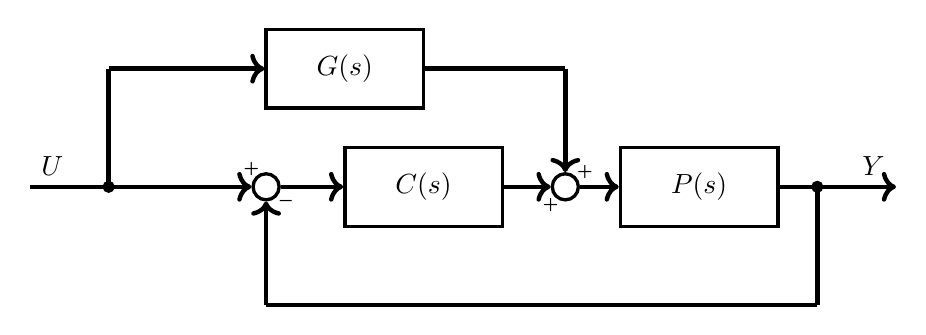
\begin{tikzpicture}[scale=2]
    \node[sum](sum)at(-1,0){};
    \draw[->,ultra thick](-1.5,0)--(sum.180)node[above]{$\scriptscriptstyle\boldsymbol{+}$};
    \filldraw[black](-2,0)circle(1pt);
    \draw[-,ultra thick](-2.5,0)node[above right]{$U$}--(-1.5,0);
    \node[block, right of=sum, node distance=2cm](c){$C(s)$};
    \node[sum]at(0.9,0)(sum2){};

    
    \draw[-,ultra thick](-2,0)--(-2,0.75);
    \node[block]at(-0.5,0.75)(g){$G(s)$};
    \draw[->,ultra thick](-2,0.75)--(g.180);
    \draw[-,ultra thick](g.0)--(0.9,0.75);
    \draw[->,ultra thick](0.9,0.75)--(sum2.90)node[right]{$\scriptscriptstyle\boldsymbol{+}$};



    \draw[->,ultra thick](sum.0)--(c.180);
    \filldraw[black](2.5,0)circle(1pt);

    \draw[->,ultra thick](2.5,0)--(3,0)node[above left]{$Y$};
    \draw[-,ultra thick](2.5,-0.75)--(2.5,0);

    %\node[block]at(0.75,-0.75)(h){$H(s)$};
    \node[block]at(1.75,0)(p){$P(s)$};

    \draw[-,ultra thick](p.0)--(2.5,0);
    \draw[->,ultra thick](c.0)--(sum2.180)node[below]{$\scriptscriptstyle\boldsymbol{+}$};
    \draw[->,ultra thick](sum2.0)--(p.180);

    %\draw[->,ultra thick](2.5,-0.75)--(h.0);
    %\draw[-,ultra thick](h.180)--(-1,-0.75);
    \draw[-,ultra thick](2.5,-0.75)--(-1,-0.75);
    \draw[->,ultra thick](-1,-0.75)--(sum.270)node[right]{$\scriptscriptstyle\boldsymbol{-}$};
\end{tikzpicture}\end{center}

\subsection{Motore a Corrente Continua}
Si vuole creare un modello per un motere elettrico, quindi si analizza il suo funzionamento. \\
Se una corrente attraversa una spira, crearà un campo magnetico, se sono 
presenti dei magneti permanenti ai lati della spira, verrà generata una forza magnetica che spinge sulla spira. Se la spira è in grado di ruotare su sé stessa, allora genererà 
un momento torcente. Per ottenere una rotazione continua bisogna invertire la corrente passante per la spira ogni mezzo giro, usando una corrente continua per ottenere ciò 
vengono usati dei contatti struscianti. In questo modo è possibile generare 
da una corrente continua e dei magneti peramnenti un momento torcente continuo. Per aumentare l'efficienza si fa ruotare il magnete all'interno di un cilindro contenete varie 
spire. Ogni volta che il magnete interno ruota di un certo angolo, si cambierà la coppia di spire che crea il campo magnetico, nonostante questo crei delle oscillazioni per 
il cambiamento di spire, la sua efficienza è notevolemente superiore ad un motore che usa contatti struscianti. \\
Si può rappresentare il circuito del rotore semplificato, formato da un'unica spira. In questo circuito semplificato sarà presente un generatore di tensione $V_a$, 
un resistore $R_a$, un induttore $L_a$, rappresentazione della spira, ed una forza contro elettro-motrice $f.c.em$, che rappresenta il magnete che ruota. 

%Ciruito in here, prova a immaginartelo eheheh. 

Per la seconda legge di Kirchoff si ottiene la seguente equazione della tensione di armatura:
\begin{equation}
    V_a=R_ai_a+L_a\dot i_a+f.c.em 
\end{equation}
La forza contro elettro-motrice generata dal magnete in rotazione è data da:
\begin{equation}
    f.c.em=\Phi_eK_a\omega\:,\:\Phi_eK_a=cost.\Rightarrow K_m=\Phi_eK_a
\end{equation}
Si avrà quindi un'equazione differenziale per la corrente, e si potrà ottenere la sua funzione di trasferimento:
\begin{gather}
    V_a=R_ai_a+L_a\dot i_a+K_m\omega\\
    V_a(s)=R_aI_a(s)+sL_aI_a(s)+K_m\Omega(s)\\
    I_a(s)=\displaystyle\frac{V_a-K_m\Omega(s)}{sL_a+R_a}
\end{gather}
Avrà un tempo caratteristico $\tau=\displaystyle\frac{1}{\displaystyle\left|\frac{R_a}{L_a}\right|}=\left|\frac{L_a}{R_a}\right|$. Questa corrente genererà una coppia 
$\tau(s)_m=K_mI_a(s)$. 
Per ottenere la rotazione del rotore bisogna esprimerla rispetto al mommento torcente prodotto. Considerando $J$ il momento di inerzia del carico, e $D$ la costante 
di attrito viscoso del rotore, si avrà:
\begin{gather}
    \tau_m(t)=J\dot\omega(t)+D\omega(t)\\
    \tau_m(s)=sJ\Omega(s)+D\Omega(s)\\
    \Omega(s)=\displaystyle\frac{\tau_m(s)}{sJ+D}
\end{gather}
Si può allora esprimere come un ciclo a controreazione:

\begin{center}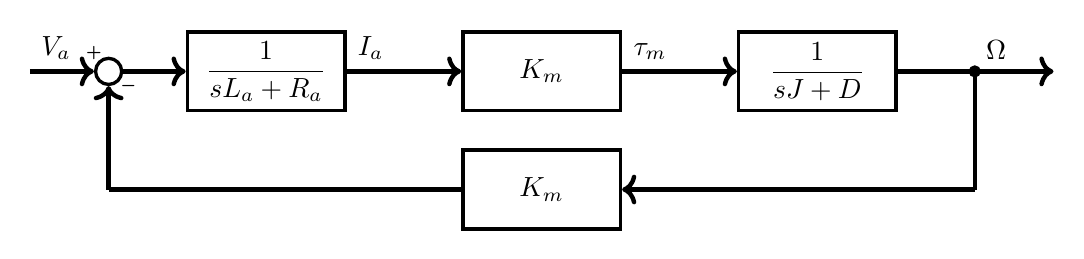
\begin{tikzpicture}[scale=2]
    \node[sum](sum)at(-1,0){};
    \draw[->,ultra thick](-1.5,0)node[above right]{$V_a$}--(sum.180)node[above]{$\scriptscriptstyle\boldsymbol{+}$};
    \node[block, right of=sum, node distance=2cm](c){$\displaystyle\frac{1}{sL_a+R_a}$};

    \draw[->,ultra thick](sum.0)--(c.180);
    \filldraw[black](4.5,0)circle(1pt);

    \draw[->,ultra thick](4.5,0)node[above right]{$\Omega$}--(5,0);
    \draw[-,ultra thick](4.5,-0.75)--(4.5,0);

    \node[block]at(1.75,-0.75)(h){$K_m$};
    \node[block]at(1.75,0)(p){$K_m$};
    \node[block]at(3.5,0)(j){$\displaystyle\frac{1}{sJ+D}$};

    \draw[->,ultra thick](p.0)node[above right]{$\tau_m$}--(j.180);
    \draw[-,ultra thick](j.0)--(4.5,0);
    \draw[->,ultra thick](c.0)node[above right]{$I_a$}--(p.180);

    \draw[->,ultra thick](4.5,-0.75)--(h.0);
    \draw[-,ultra thick](h.180)--(-1,-0.75);
    %\draw[-,ultra thick](2.5,-0.75)--(-1,-0.75);
    \draw[->,ultra thick](-1,-0.75)--(sum.270)node[right]{$\scriptscriptstyle\boldsymbol{-}$};
\end{tikzpicture}\end{center}
Per ottenere l'angolo al posto della velocità angolare del rotore, si può inserire un integratore $\displaystyle\frac{1}{s}$ sull'uscita $\Omega$. Per ottenere una velocità 
maggiore bisognerà allora aumentare il guadagno della funzione di trasferimento a ciclo chiuso $W(s)$. 

\subsection{Controllori}

Un controllore è un oggetto fisico usato per manipolare la stabilità di un sistema, il suo comportamento nel transitorio e a pieno regime. 
Esistono vari tipi di controllori, il più semplice è un controllore proporzionale che consiste di una costante $K_c$ che moltiplica l'ingresso, in modo 
che il processo lavori su un'entrata $Kc\cdot U$, se il controllore proporzionale vale $1$, avrà guadagno unitario. Per ottenere della catena 
diretta si moltiplica il guadagno del controllore, per il guadagno del processo: $K=K_c\cdot K_P$. Considerando un processo 
$P(s)=\displaystyle\frac{N(s)}{D(s)}$, si avrà una funzione a ciclo chiuso, per un controllore proporzionale: 

\begin{equation}
    W(s)=\displaystyle\frac{Kc\displaystyle\frac{N(s)}{D(s)}}{1+Kc\displaystyle\frac{N(s)}{D(s)}}=\frac{K_cN(s)}{D(s)+K_cN(s)}
\end{equation}

\begin{center}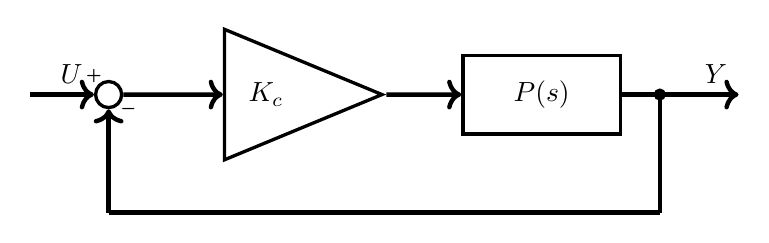
\begin{tikzpicture}[scale=2]
    \node[sum](sum)at(-1,0){};
    \draw[->,ultra thick](-1.5,0)--(sum.180)node[above left]{$U$}node[above]{$\scriptscriptstyle\boldsymbol{+}$};
    \node[triangle, right of=sum, node distance=2cm](c){$K_c$};

    \draw[->,ultra thick](sum.0)--(c.180);
    \filldraw[black](2.5,0)circle(1pt);

    \draw[->,ultra thick](2.5,0)--(3,0)node[above left]{$Y$};
    \draw[-,ultra thick](2.5,-0.75)--(2.5,0);

    %\node[block]at(0.75,-0.75)(h){$H(s)$};
    \node[block]at(1.75,0)(p){$P(s)$};

    \draw[-,ultra thick](p.0)--(2.5,0);
    \draw[->,ultra thick](c.0)--(p.180);

    %\draw[->,ultra thick](2.5,-0.75)--(h.0);
    %\draw[-,ultra thick](h.180)--(-1,-0.75);
    \draw[-,ultra thick](2.5,-0.75)--(-1,-0.75);
    \draw[->,ultra thick](-1,-0.75)--(sum.270)node[right]{$\scriptscriptstyle\boldsymbol{-}$};
\end{tikzpicture}\end{center}

\subsubsection{Luogo delle Radici}

Il teorema sulla continuità delle radici di un polinomio descrive il comportamento delle soluzioni di un polinomio, alterando leggermente i 
valori dei coefficienti del polinomio:
\begin{quotation}
    Considerando un polinomio $P^n(x)=a_nx^n+...a_1x=0$, sarà sempre possibile trovare una soluzione $x_0'$ nell'intorno $I_{\varepsilon}(x_0)$, dove $x_0$ 
    è una soluzione di $P(x)$, al polinomio $P'(x)=(a_n+\varepsilon)x^n+...(a_1+\varepsilon)x=0$, per ogni $\varepsilon>0$ scelto arbitrariammente. 
\end{quotation} 
Per cui se esiste almeno una soluzione di $D(s)+K_cN(s)$, allora sarà sempre possibile trovare una sua soluzione per ogni valore di $K_c$ scelto. 
Per valori di $K_c\approx0$, si potrà approssimare il denominatore a: $D(s)+K_cN(s)\approx D(s)$, quindi il valore dei poli sarà dato dalla sola 
funzione $D(s)$, al contrario per valori del guadagno del controllore molto elevati  $K_c>>0$, si avrà $D(s)+K_cN(s)\approx N(s)$, quindi il valore 
dei poli sarà dato dalla sola funzione $N(s)$. 
Per controllare l'andamento dei poli della funzione a ciclo chiuso rispetto ai valori del guadagno del controllore, si usa il luogo delle radici, un 
grafico che che mostra lo spostamento dei poli rispetto all'aumento del guadadno, i poli partiranno dai valori dei poli del processo, fino a tendere 
al valore degli zeri del processo. Se il processo presenta un numero minore di zeri, allora alcuni dei poli tenderanno all'infinito. 
Il luogo della radici viene rappresentato su un piano di Gauss. Se due poli sono complessi e coinugati, allora il loro comportamento rispetto all'
aumentare del guadagno sarà simmetrico. Questi poli possono essere espressi come: 
\begin{equation}
    (s+p_1)(s+p_1^*)=\displaystyle\frac{s^2}{\omega_0^2}+\frac{2\xi}{\omega_0}s+1
\end{equation}
Dove $\xi$ rappresenta lo smorzamento del polo, quantifica quanto persiste l'oscillazione del sistema in seguito ad un dato ingresso, è dato da 
$\xi=cos\varphi$, dove $\varphi$ rappresenta l'angolo con l'orizzontale rispetto a $\omega_0$, la distanza tra l'origne $O$ ed il polo, che esprime 
l'ampiezza dell'oscillazione. 
Per cui il polo espresso in coordinate polari sarà $(\omega_0,\:\varphi)$. 
Un polo con uno smorzamento maggiore tenderà a convergere più velocemente, e avrà un tempo caratteristico minore. \\
In matalab si può ottenere il grafico del luogo delle radici per qualsiasi funzione di trasferimento tramite il comando 
La funzione di trasferimento sarà stabile se il luogo delle radici è intermaente nel semipiano di parte reale negativa, altrimenti sarà stabile solo 
in un certo intervallo di $K_c$. La funzione "rlocus(F)" analizza solo valori positivi del guadagno, per controllare se l'intervallo si estenda anche per 
valori negativi bisogna controllare "rlocus(-F)". Le linee radiali uscenti dall'origine rappresentano le linee di smorzamento. 
I punti segnati con una croce rappresetano i poli, mentre i punti indiviuati da un cerchio rappresentano gli zeri della funzione.\\
Aumentando il guadagno, aumenta l'ampiezza di un'oscillazione e diminuisce l'errore che ne deriva. La robustezza di un sistema è una misura che 
quantifica quanto un sistema mantiene nel sue dinamiche nel tempo, rispetto ad errori. 

\begin{center}
    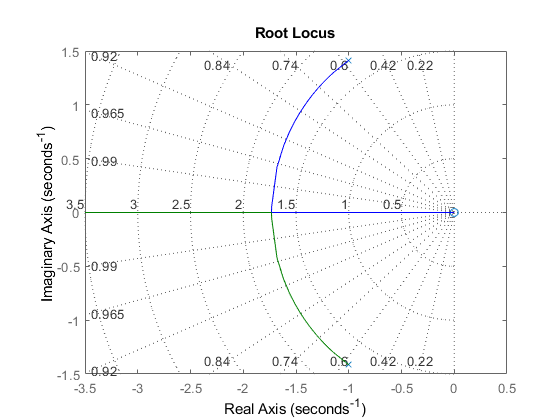
\includegraphics[scale=0.55]{rlocus}
    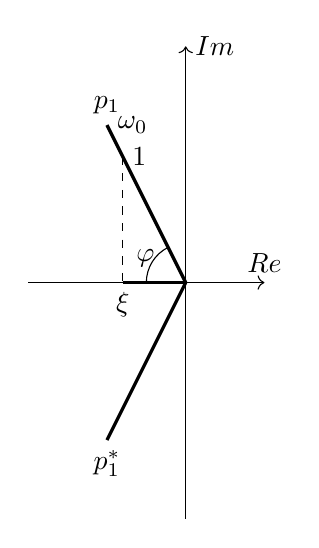
\begin{tikzpicture}[scale=2]
    \coordinate(O)at(0,0);
    \draw[->](-1,0)coordinate(Re)--(0.5,0)node[above]{$Re$};
    \draw[->](0,-1.5)--(0,1.5)coordinate(Im)node[right]{$Im$};

    \draw[-,very thick](O)--(-0.5,1)coordinate(w)node[right]{$\omega_0$}node[above]{$p_1$};
    \draw[-,very thick](O)--(-0.5,-1)node[below]{$p_1^*$};
    \draw[dashed](-0.4,0.8)node[right]{$1$}--(-0.4,0)node[below]{$\xi$};
    \draw[-,thick](-0.4,0)--(0,0);
    \pic["$\varphi$",draw, angle eccentricity=1.2, angle radius=0.5cm]{angle=w--O--Re};

    \end{tikzpicture}
\end{center}

\subsubsection{Controllore Proporzionale con un integratore}
Per controllare l'effetto di un controllore proporzionale sul guadadno di un sistema, si considera un'entrata a gradino $U(s)=\displaystyle\frac{1}{s}$, e si calcola con 
il teorma del valore finale il valore dell'uscita a regime permanente:
\begin{gather}
    W(s)=\displaystyle\frac{Y(s)}{U(s)}=\frac{K_cN(s)}{D(s)+K_cN(s)}\\
    Y(s)=\displaystyle\frac{K_c N(s)}{D(s)+K_c N(s)}\frac{1}{s}\\
    K_Y=\lim_{s\to0}s\cdot Y(s)=\lim_{s\to0}s\displaystyle\frac{K_c N(s)}{D(s)+K_c N(s)}\frac{1}{s}\\
    K_Y=\displaystyle\frac{K_c}{\displaystyle\frac{1}{K_P}+K_c}<1
\end{gather}
Dove $K_P$ è il guadagno del proceso $P(s)$. Per valori piccoli di $K_c$, si avrà un errore $e_Y=1-K_Y$ elevato, solo all'umentare di $K_c$ l'errore diminuirà fino a tendere 
a $1$ per $K_c\to\infty$: 
\begin{equation}
    e_Y=1-\lim_{K_c\to\infty}\displaystyle\frac{K_c}{\displaystyle\frac{1}{K_P}+K_c}=1-1=0
\end{equation}
Si vuole ottenere un'errore nullo senza aumentare il guadagno $K_c$, poiché cambierebbe l'andamento del processo nel transitorio. Inserendo un integratore insieme ad 
un controllore proporzionale $\displaystyle\frac{K_c}{s}$ si avrà una funzione a ciclo chiuso:
\begin{equation}
    W(s)=\displaystyle\frac{K_cN(s)}{sD(s)+K_cN(s)}
\end{equation}
Il guadagno dell'uscita per un'entrata a gradino sarà in questo caso:
\begin{equation}
    K_Y=\lim_{s\to0}s\displaystyle\frac{K_c N(s)}{sD(s)+K_c N(s)}\frac{1}{s}=\frac{K_c}{0\cdot\displaystyle\frac{1}{K_P}+K_c}=1
\end{equation}
Si può quindi ottenere un'errore nullo a regime permanente, indipendentemente dal valore del controllore prooprzionale. Da notare come per ottenere un errore nullo è stato 
necessario inserire un integratore, per un'entrata a gradino. Per il principio del modello interno per ottenere un'uscita di un certo tipo sarà necessaria una dinamica 
simile all'initerno del sistema. Segue che per un sistema asintoticamente stabile, l'uscita seguirà l'entrata, ovvero entrambe saranno dello stesso tipo. 

\begin{center}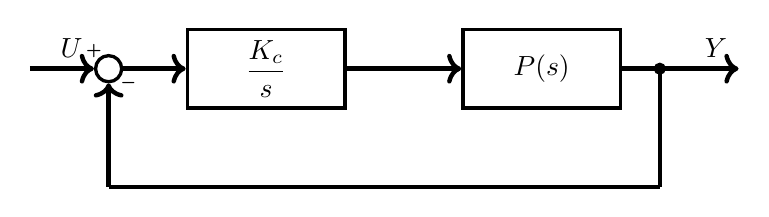
\begin{tikzpicture}[scale=2]
    \node[sum](sum)at(-1,0){};
    \draw[->,ultra thick](-1.5,0)--(sum.180)node[above left]{$U$}node[above]{$\scriptscriptstyle\boldsymbol{+}$};
    \node[block, right of=sum, node distance=2cm](c){$\displaystyle\frac{K_c}{s}$};

    \draw[->,ultra thick](sum.0)--(c.180);
    \filldraw[black](2.5,0)circle(1pt);

    \draw[->,ultra thick](2.5,0)--(3,0)node[above left]{$Y$};
    \draw[-,ultra thick](2.5,-0.75)--(2.5,0);

    %\node[block]at(0.75,-0.75)(h){$H(s)$};
    \node[block]at(1.75,0)(p){$P(s)$};

    \draw[-,ultra thick](p.0)--(2.5,0);
    \draw[->,ultra thick](c.0)--(p.180);

    %\draw[->,ultra thick](2.5,-0.75)--(h.0);
    %\draw[-,ultra thick](h.180)--(-1,-0.75);
    \draw[-,ultra thick](2.5,-0.75)--(-1,-0.75);
    \draw[->,ultra thick](-1,-0.75)--(sum.270)node[right]{$\scriptscriptstyle\boldsymbol{-}$};
\end{tikzpicture}\end{center}

\subsubsection{Entrata di Tipo $k$}

Poiché l'uscita tenderà a seguire l'entrata, si considera un modello di riferimento ideale, dove l'uscita $Y_d$ è proporzionale all'entrata di un fattore $K_d$:
\begin{equation}
    Y_d=K_d\cdot U\Rightarrow W_d(s)=K_d
\end{equation}
Ma non potrà esistere un sistema fisico tale da avere una funzione a ciclo chiuso uguale ad una costante. Per cui si vuole calcolare l'errore di un sistema rispetto a 
questo riferimento ideale, per ottenerlo si considera: 

\begin{center}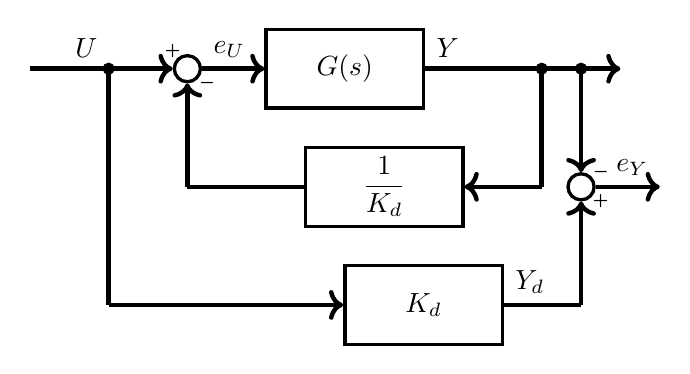
\begin{tikzpicture}[scale=2]
    \node[sum](sum)at(-1,0){};
    \draw[->,ultra thick](-1.5,0)--(sum.180)node[above]{$\scriptscriptstyle\boldsymbol{+}$};
    \draw[-,ultra thick](-2,0)--(-1.5,0)node[above left]{$U$};
    \filldraw[black](-1.5,0)circle(1pt);
    %\node[triangle, right of=sum, node distance=2cm](c){$K_c$};

    %\draw[->,ultra thick](sum.0)--(c.180);
    \filldraw[black](1.25,0)circle(1pt);
    \filldraw[black](1.5,0)circle(1pt);
    \draw[-,ultra thick](1.25,0)--(1.5,0);
    \draw[->,ultra thick](1.5,0)--(1.75,0);

    %\draw[->,ultra thick](2.5,0)--(3,0)node[above left]{$Y$};
    %\draw[-,ultra thick](2.5,-0.75)--(2.5,0);

    \node[block]at(0.25,-0.75)(h){$\displaystyle\frac{1}{K_d}$};
    \node[block, right of=sum, node distance=2cm](p){$G(s)$};
    \draw[->,ultra thick](sum.0)node[above right]{$e_U$}--(p.180);
    \draw[-,ultra thick](p.0)node[above right]{$Y$}--(1.25,0);
    %\draw[->,ultra thick](c.0)--(p.180);

    \draw[-,ultra thick](1.25,0)--(1.25,-0.75);
    \draw[->,ultra thick](1.25,-0.75)--(h.0);
    \draw[-,ultra thick](h.180)--(-1,-0.75);
    %\draw[-,ultra thick](2.5,-0.75)--(-1,-0.75);
    \draw[->,ultra thick](-1,-0.75)--(sum.270)node[right]{$\scriptscriptstyle\boldsymbol{-}$};

    \node[sum](sum2)at(1.5,-0.75){};
    \draw[->,ultra thick](1.5,0)--(sum2.90)node[right]{$\scriptscriptstyle\boldsymbol{-}$};
    \node[block](k)at(0.5,-1.5){$K_d$};
    \draw[-,ultra thick](k.0)node[above right]{$Y_d$}--(1.5,-1.5);
    \draw[->,ultra thick](1.5,-1.5)--(sum2.270)node[right]{$\scriptscriptstyle\boldsymbol{+}$};

    \draw[-,ultra thick](-1.5,0)--(-1.5,-1.5);
    \draw[->,ultra thick](-1.5,-1.5)--(k.180);

    \draw[->,ultra thick](sum2.0)--(2,-0.75)node[above left]{$e_Y$};

\end{tikzpicture}\end{center}

Si avrà quindi un errore in entrata $e_U$ dovuto alla differenza tra la funzione a ciclo chiuso ed il modello ideale: 
\begin{equation}
    e_U=U-\displaystyle\frac{Y}{K_d}
\end{equation}
questo errore sarà nullo per valori di uscita uguali al riferimento ideale: $Y=Y_d=K_dU$.\\
Si avrà un errore in uscita:
\begin{gather}
    e_Y:E(s)=Y_d-Y=K_dU(s)-W(s)U(s)\\
    K_dU(s)-\displaystyle\frac{K_dG(s)}{K_d+G(s)}U(s)\\
    \left(\displaystyle\frac{K_d^2+K_dG(s)-K_dG(s)}{K_d+G(s)}\right)U(s)\\
    E(s)=\displaystyle\frac{K_d^2}{K_d+G(s)}U(s)
\end{gather}
Per cui è necessario conoscere l'ingresso del sistema per poter determinare l'errore in uscita. Si analizza il caso di entrate del tipo $k$ polinomiale: 
\begin{equation}
    u(t)=\displaystyle\frac{t^k}{k!}=\delta_{-(k+1)}(t)\Rightarrow U(s)=\displaystyle\frac{1}{s^{k+1}}
\end{equation}
Si considera il processo $G(s)$ contente un numero $h$ di integratori:
\begin{equation}
    G(s)=\displaystyle\frac{G'(s)}{s^h}
\end{equation}

Allora si avrà un errore in uscita:
\begin{equation}
    E(s)=\displaystyle\frac{K_d^2}{K_d+\displaystyle\frac{G'(s)}{s^h}}\frac{1}{s^{(k+1)}}
\end{equation}
Si vuole determinare per quali valore di $h$ si ha un errore nullo a regime permanetne, per cui si analizza: 
\begin{equation}
    \lim_{s\to0}s\cdot E(s)=\lim_{s\to0}s\cdot\displaystyle\frac{K_d^2}{K_d+\displaystyle\frac{G'(s)}{s^h}}\frac{1}{s^{(k+1)}}=\frac{K_d^2}{G'(0)}\lim_{s\to0}\frac{1}{s^{k-h}}
\end{equation}
Si definisce guadagno generalizzato $K_G$ di una funzione $G(s)=\displaystyle\frac{G'(s)}{s^h}$, il suo valore per $s=0$, senza considerare gli integratori, per cui: $K_G=G'(0)$. 
Per cui l'errore in uscita e pieno regime dipenderà dal numero di integratori nel processo $G$:
\begin{equation}
    \displaystyle\frac{K_d^2}{K_G}\lim_{s\to0}\frac{1}{s^{k-h}}=
    \begin{cases}
        +\infty,\:k>h\\
        \displaystyle\frac{K_d^2}{K_G},\:k=h\\
        0,\:k<h
    \end{cases}
\end{equation}
Segue che per rigettare un errore di tipo $k$, serviranno $k$ integratori nella catena diretta. Anche se inserire un numero maggiore di integratori annulla l'errore, non è 
consigliato inserire un numero maggiore dell'indispensabile di integratori nella catena diretta, poiché più aumenta il numero di poli nell'origine più il sistema tende all'
instabilità. Viene definito sistema di controllo di tipo $k$, un controllore tale da rendere l'errore a regime permanente costante per un'entrta di tipo $k$. Da notare che 
per un entrata di tipo $0$, non serviranno integratori e l'errore a regime permanente sarà dato da: $E_Y=\displaystyle\frac{K_d^2}{K_d+K_G}$. \'{E} possibile quindi 
creare una tabella che mostri l'andamento dell'errore rispetto ad entrate di tipo $k$ e un numero $h$ di integratori in catena diretta:

\begin{center}
    \begin{tabular}{|c|c|c|c|c}
        \hline
        $h,\:k$ & $0$ & $1$ & $2$ & $\ldots$\\[0.5ex]
        \hline
        $0$ & $\displaystyle\frac{K_d^2}{K_d+K_G}$ & $\infty$ &$\infty$\\[0.5ex]
        \hline
        $1$ & $0$ & $\displaystyle\frac{K_d^2}{K_G}$ & $\infty$\\[0.5ex]
        \hline
        $2$ & $0$ & $0$ & $\displaystyle\frac{K_d^2}{K_G}$\\[0.5ex]
        \hline
        $\vdots$ & & & & $\ddots$\\
    \end{tabular}
\end{center}

\begin{center}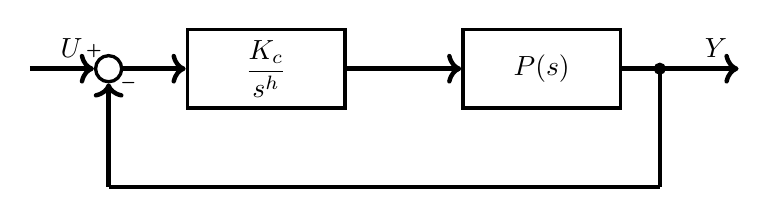
\begin{tikzpicture}[scale=2]
    \node[sum](sum)at(-1,0){};
    \draw[->,ultra thick](-1.5,0)--(sum.180)node[above left]{$U$}node[above]{$\scriptscriptstyle\boldsymbol{+}$};
    \node[block, right of=sum, node distance=2cm](c){$\displaystyle\frac{K_c}{s^h}$};

    \draw[->,ultra thick](sum.0)--(c.180);
    \filldraw[black](2.5,0)circle(1pt);

    \draw[->,ultra thick](2.5,0)--(3,0)node[above left]{$Y$};
    \draw[-,ultra thick](2.5,-0.75)--(2.5,0);

    %\node[block]at(0.75,-0.75)(h){$H(s)$};
    \node[block]at(1.75,0)(p){$P(s)$};

    \draw[-,ultra thick](p.0)--(2.5,0);
    \draw[->,ultra thick](c.0)--(p.180);

    %\draw[->,ultra thick](2.5,-0.75)--(h.0);
    %\draw[-,ultra thick](h.180)--(-1,-0.75);
    \draw[-,ultra thick](2.5,-0.75)--(-1,-0.75);
    \draw[->,ultra thick](-1,-0.75)--(sum.270)node[right]{$\scriptscriptstyle\boldsymbol{-}$};
\end{tikzpicture}\end{center}

\subsubsection{Disturbo di Tipo $k$}

Nel caso sia presente un disturbo di tipo $k$ sulla catena diretta $z(t)=\delta_{-(k+1)}(t)$, per rigettarlo a regime permanente bisogna ottenere un'errore nullo in uscita 
considerando il disturbo come unica entrata del sistema. 

\begin{center}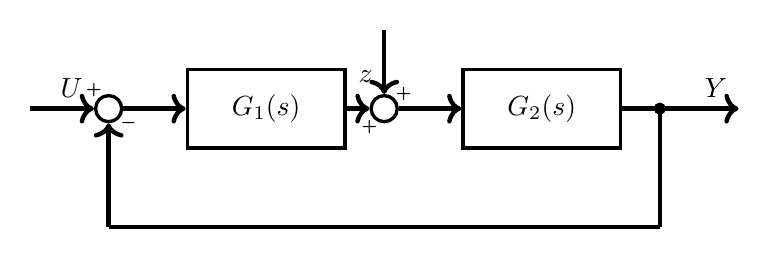
\begin{tikzpicture}[scale=2]
    \node[sum](sum)at(-1,0){};
    \node[sum](sum2)at(0.75,0){};
    \draw[->,ultra thick](-1.5,0)--(sum.180)node[above left]{$U$}node[above]{$\scriptscriptstyle\boldsymbol{+}$};


    \node[block, right of=sum, node distance=2cm](g){$G_1(s)$};
    \draw[->,ultra thick](sum.0)--(g.180);
    \draw[->,ultra thick](g.0)--(sum2.180)node[below]{$\scriptscriptstyle\boldsymbol{+}$};
    

    \filldraw[black](2.5,0)circle(1pt);


    \draw[->,ultra thick](0.75,0.5)--(sum2.90)node[above left]{$z$}node[right]{$\scriptscriptstyle\boldsymbol{+}$};

    \node[block]at(1.75,0)(k){$G_2(s)$};
    \draw[->,ultra thick](sum2.0)--(k.180);
    \draw[-,ultra thick](k.0)--(2.5,0);

    \draw[->,ultra thick](2.5,0)--(3,0)node[above left]{$Y$};
    \draw[-,ultra thick](2.5,-0.75)--(2.5,0);


    %\node[block, below of=g, node distance=1.5cm](h){$H(s)$};
    %\draw[->,ultra thick](1.25,-0.75)--(h.0);
    %\draw[-,ultra thick](h.180)--(-1,-0.75);
    \draw[-,ultra thick](2.5,-0.75)--(-1,-0.75);
    \draw[->,ultra thick](-1,-0.75)--(sum.270)node[right]{$\scriptscriptstyle\boldsymbol{-}$};
\end{tikzpicture}\end{center}

Allora si avrà una funzione a ciclo chiuso del disturbo:
\begin{equation}
    W_z(s)=\displaystyle\frac{G_2(s)}{1+G_1(s)G_2(s)}
\end{equation}
Ed un'uscita a regime permanente $Y_z$:
\begin{equation}
    Y_z=\lim_{s\to0}s\cdot\displaystyle\frac{G_2(s)}{1+G_1(s)G_2(s)}\frac{1}{s^{k+1}}
\end{equation}
Per poter rigettare il disturbo bisogna inserire $k$ integratori a monte di esso, ovvero nella funzione $G_1(s)$, l'errore causato a regime permanente allora sarà:
\begin{gather}
    Y_z=\lim_{s\to0}s\cdot\displaystyle\frac{G_2(s)}{1+\displaystyle\frac{G_1'(s)}{s^k}G_2(s)}\frac{1}{s^{k+1}}=\frac{K_{G_2}}{K_{G_1}K_{G_2}}
\end{gather}

Per cui per inseguire o rigettare un polinomio di tipo $k$ in entrata, servono $k$ integratori in catena diretta, a monte del disturbo. Gli integratori nella funzinoe $G_1$ 
annulano l'errore per un entrata di tipo $k$ e rigettano un disturbo di tipo $k$. Ma l'inserimento di poli nell'orgine 
destabilizza il sistema, quindi è necessario inserire un altro elemento per recuperare la stabilità. \\ 

Considerando il motore a corrente diretta, un possible disturbo potrebbe essere il peso del carico che sta spostando che produrra un momento torcente costante nel tempo, 
per cui sarà un disturbo di tipo $0$ e necessiterà di un controllore di tipo $0$ a monte del disturbo. Nel caso di un motore, si considera un riferimento ideale legato da 
una cosante unitaria: $Y_d=U$, ovvero per una qualsiasi entrata, l'uscita la deve seguire esattamente. Per cui l'errore risultarà: $e=\displaystyle\frac{1}{1+K_cK_{DC}}$, 
dove $K_c$ è il guadagno del controllore di tipo $0$. Se il motore opera dei sistemi precisi, richiederanno un'errore nullo 
indipendentemente dal valore del guadagno del controllore quindi si userà un controllore di tpo $1$, ma ciò renderà il transitorio molto lungo, poiché un integratore 
prima di diventare utile dovrà caricarsi per un certo intervallo di tempo, prima di agire come richiesto. Ciò altererà i punti di equilibrio del rotore, ma inserire un 
altro integratore per rigettare l'errore renderebbe il sistema instabile, per cui si può alterare manualmente il riferimento iniziale su cui opera il sistema. 

\begin{center}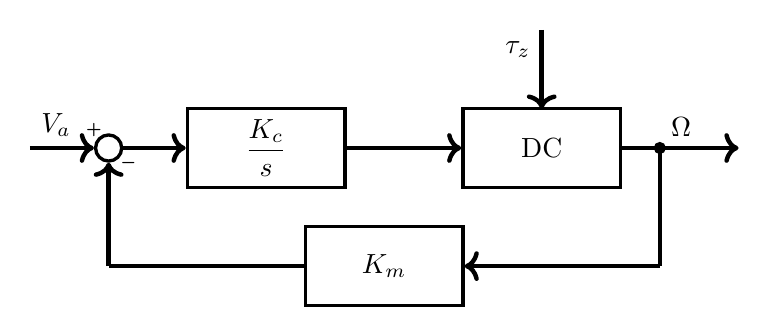
\begin{tikzpicture}[scale=2]
    \node[sum](sum)at(-1,0){};
    \draw[->,ultra thick](-1.5,0)node[above right]{$V_a$}--(sum.180)node[above]{$\scriptscriptstyle\boldsymbol{+}$};
    \node[block, right of=sum, node distance=2cm](c){$\displaystyle\frac{K_c}{s}$};

    \draw[->,ultra thick](sum.0)--(c.180);
    \filldraw[black](2.5,0)circle(1pt);

    \draw[->,ultra thick](2.5,0)node[above right]{$\Omega$}--(3,0);
    \draw[-,ultra thick](2.5,-0.75)--(2.5,0);

    \node[block]at(0.75,-0.75)(h){$K_m$};
    \draw[->,ultra thick](1.75,0.75)node[below left]{$\tau_z$}--(1.75,0.25);
    \node[block]at(1.75,0)(p){DC};

    \draw[-,ultra thick](p.0)--(2.5,0);
    \draw[->,ultra thick](c.0)--(p.180);

    \draw[->,ultra thick](2.5,-0.75)--(h.0);
    \draw[-,ultra thick](h.180)--(-1,-0.75);
    %\draw[-,ultra thick](2.5,-0.75)--(-1,-0.75);
    \draw[->,ultra thick](-1,-0.75)--(sum.270)node[right]{$\scriptscriptstyle\boldsymbol{-}$};
\end{tikzpicture}\end{center}

\subsubsection{Controllore Proporzionale, Integrativo e Derivativo (PID)}

Considerando l'errore in uscita nel dominio del tempo $e(t)=u(t)-y(t)$, assumendo un ingresso costante si avrà: $\dot e(t)=-\dot y(t)\Rightarrow sE(s)=-sK_dY(s)$, 
un derivatore agirà su questa componente dell'errore agendo come un riduttore, ovvero come una forma di attrito, annullandolo. Questo procedimento 
però non funzionerà per ogni sistema, è possible che un sistema abbia troppo attrito, quindi un riduttore non porterebbe effetti desiderati, agendo su quel sistema. 
Per cui per alcuni sistema inserire un derivatore può aiutare nel loro controllo. \\
Un controllore che contiene un parametro proporzionale 
integrativo e derivativo viene chiamato controllore PID. L'oggetto fisico può escludere il cavo di riferimento, poiché può essere computato. 

\begin{center}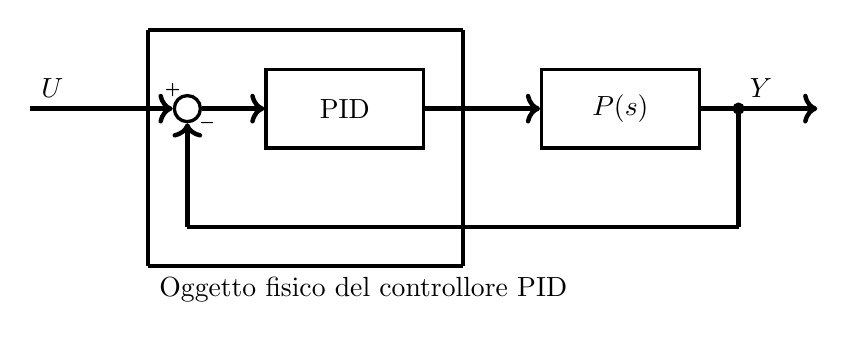
\begin{tikzpicture}[scale=2]
    \node[sum](sum)at(-1,0){};
    \draw[->,ultra thick](-2,0)node[above right]{$U$}--(sum.180)node[above]{$\scriptscriptstyle\boldsymbol{+}$};
    \node[block, right of=sum, node distance=2cm](c){PID};

    \draw[-,ultra thick](0.75,0.5)--(0.75,-1);
    \draw[-,ultra thick](0.75,0.5)--(-1.25,0.5);
    \draw[-,ultra thick](0.75,-1)--(-1.25,-1);
    \draw[-,ultra thick](-1.25,0.5)--(-1.25,-1)node[below right]{Oggetto fisico del controllore PID};

    \draw[->,ultra thick](sum.0)--(c.180);
    \filldraw[black](2.5,0)circle(1pt);

    \draw[->,ultra thick](2.5,0)node[above right]{$Y$}--(3,0);
    \draw[-,ultra thick](2.5,-0.75)--(2.5,0);

    %\node[block]at(0.75,-0.75)(h){$H(s)$};
    \node[block]at(1.75,0)(p){$P(s)$};

    \draw[-,ultra thick](p.0)--(2.5,0);
    \draw[->,ultra thick](c.0)--(p.180);

    %\draw[->,ultra thick](2.5,-0.75)--(h.0);
    %\draw[-,ultra thick](h.180)--(-1,-0.75);
    \draw[-,ultra thick](2.5,-0.75)--(-1,-0.75);
    \draw[->,ultra thick](-1,-0.75)--(sum.270)node[right]{$\scriptscriptstyle\boldsymbol{-}$};
\end{tikzpicture}\end{center}


Un controllore PID sarà quindi un 
oggetto avente funzione di trasferimento: $K_c+K_i\displaystyle\frac{1}{s}+K_ds$. Poiché un derivatore è un oggetto non causale, dipendendo da entrate future, si 
inserisce un polo lontano in un valore 
$\displaystyle\frac{1}{\varepsilon}$, per $\varepsilon$ arbitrariamente piccolo, in modo che risenta del polo solo per valori molto alti. Per cui la parte derivativa sarà: 
$\displaystyle\frac{K_ds}{s\varepsilon+1}$, si può esprimere come: 
$\displaystyle\frac{K_ds}{s\varepsilon+1}\frac{\displaystyle\frac{1}{s\varepsilon}}{\displaystyle\frac{1}{s\varepsilon}}=\frac{K_dN}{1+\displaystyle\frac{N}{s}}$, dove 
$N$ rappresenta un valore arbitrariamente grande. Un controllore PID può essere espresso, esplicitando il suo guadano come: 
\begin{equation}
    PID(s)=K_p\left(1+K_i\displaystyle\frac{1}{s}+K_d\frac{N}{1+\displaystyle\frac{N}{s}}\right)
\end{equation}
Per costruire un derivatore si considera: 

\begin{center}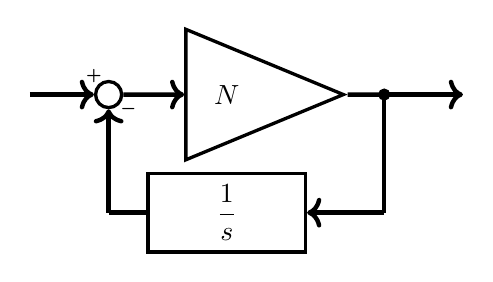
\begin{tikzpicture}[scale=2]
    \node[sum](sum)at(-1,0){};
    \draw[->,ultra thick](-1.5,0)--(sum.180)node[above]{$\scriptscriptstyle\boldsymbol{+}$};
    \node[triangle, right of=sum, node distance=1.5cm](g){$N$};
    \draw[->,ultra thick](sum.0)--(g.180);
    \draw[-,ultra thick](g.0)--(0.75,0);
    \filldraw[black](0.75,0)circle(1pt);
    \draw[->,ultra thick](0.75,0)--(1.25,0);
    \draw[-,ultra thick](0.75,-0.75)--(0.75,0);
    \node[block, below of=g, node distance=1.5cm](h){$\displaystyle\frac{1}{s}$};
    \draw[->,ultra thick](0.75,-0.75)--(h.0);
    \draw[-,ultra thick](h.180)--(-1,-0.75);
    \draw[->,ultra thick](-1,-0.75)--(sum.270)node[right]{$\scriptscriptstyle\boldsymbol{-}$};
\end{tikzpicture}\end{center}

Quest'oggetto fisicamente realizzabile avrà una funzione a ciclo chiuso $W(s)=\displaystyle\frac{N}{1+\displaystyle\frac{N}{s}}$, per un guadadno sulla catena diretta 
tendente all'infinito $N\to\infty$, si avrà un derivatore puro. 


\clearpage 

\section{Ingressi di Tipo Sinusoidale}

Per degli ingressi del tipo $u(t)=sin(\omega t)$, si ipotizza che un processo $G(s)$ sia asintoticamente stabile, e quindi abbia un'uscita a regime permanente della stessa 
classe dell'ingresso, ovvero $y_p(t)=Asin(\Omega t)$. La risposta del sistema nel dominio di Laplace sarà data da: 
$Y_p(s)=G(s)\cdot\displaystyle\frac{\omega}{s^2+\omega^2}$, si potrà scomporre in poli residui come: $Y_p(s)=\displaystyle\frac{R}{s-j\omega}+\frac{R^*}{s+j\omega}$, i valori 
di $R$ potranno essere calcolati usando la formula dei poli residui: 
\begin{gather}
    R=\lim_{s\to j\omega}(s-j\omega)Y_p(s)=\lim_{s\to j\omega}(s-j\omega)G(s)\cdot\displaystyle\frac{\omega}{s^2+\omega^2}\\
    \lim_{s\to j\omega}\cancelto{1}{(s-j\omega)}G(s)\displaystyle\frac{\omega}{\cancelto{1}{(s-j\omega)}(s+j\omega)}\\
    R=\displaystyle\frac{G(j\omega)\omega}{2j\omega}=\frac{G(j\omega)}{2j}\\
    R^*=-\frac{G^*(j\omega)}{2j}
\end{gather}
La funzione $G(j\omega)$, può essere espressa in termini polari come:
\begin{gather}
    G(j\omega)=|G(j\omega)|e^{j\phase{G(j\omega)}}\\
    G^*(j\omega)=|G(j\omega)|e^{-j\phase{G(j\omega)}}
\end{gather}

Allora si potrà esprimere la risposta a regime permanente come:
\begin{gather}
    Y_p(s)=\displaystyle\frac{1}{2j}\left(\frac{G(j\omega)}{s-j\omega}-\frac{G^*(j\omega)}{s+j\omega}\right)\\
    y_p(y)=\displaystyle\frac{1}{2j}(G(j\omega)e^{j\omega t}-G^*(j\omega)e^{-j\omega t})\\
    \displaystyle\frac{1}{2j}\left(|G(j\omega)|e^{j\phase{G(j\omega)}}e^{j\omega t}-|G(j\omega)|e^{-j\phase{G(j\omega)}}e^{-j\omega t}\right)\\
    |G(j\omega)|\left(\displaystyle\frac{e^{j\left(\omega t+\phase{G(j\omega)}\right)}-e^{-j\left(\omega t+\phase{G(j\omega)}\right)}}{2j}\right)\\
    y_p(t)=|G(j\omega)|sin\left(\omega t+\phase{G(j\omega)}\right)
\end{gather}

La risposta è proporzionale al modulo $|G(j\omega)|$. Data una certa pulsazione si ha che la risposta si annulla, per poi diventare negativa, per cui non si può 
amplificare una frequenza all'infinito. 

\begin{center}
    \begin{tikzpicture}[scale=2]
        \draw[->](0,-0.5)--(0,2)node[right]{$y_p(t)$};
        \draw[->](-0.5,0)--(2,0)node[above]{$\omega$};

        \draw[-, very thick]plot[smooth, domain=0:1.5](\x,{(1.5-\x)^0.5});
        \node[below]at(1.5,0){$\omega_t$};
    \end{tikzpicture}
\end{center}

Quest'analisi coincide con una trasformata di Fuorier, poiché una trasformata di Fuorier non è altro che una trasformata di Laplace solamente sull'asse 
immaginario: \\$\displaystyle\mathscr{F}_-(g(t))=\int_{0}^{\infty}g(t)e^{-j\omega t}dt=\mathscr{L}_-(y_p(t))\bigg|_{s=j\omega}$, corrisponde ad un'analisi dei soli segnali periodici. 
Per analizzare il comportamento della risposta del sistema, si dovranno analizzare gli andamenti del modulo e della fase del processo rispetto ad una pulsazione $\omega$. 

\subsection{Diagrammi di Bode}

Per analizzare il modulo di una funzione $G(s)$, con un guadagno normalizzato:
\begin{equation}
    G(s)=K_g\displaystyle\frac{(s\tau_i+1)\ldots(s\tau_n+1)}{(s\tau_k+1)\ldots(s\tau_m+1)}
\end{equation}
Per facilitare l'analisi rispetto ad ogni polo della funzione si considera una scala logaritimica in Decbibel:
\begin{equation}
    \big|x\big|_{dB}=20\log_{10}|x|
\end{equation}
Il modulo in Decibel del guadagno della funzione $K_g$, risulterà una costante addittiva:
\begin{equation}
    \big|K_g\big|_{dB}=20\log_{10}|K_g|
\end{equation}
Per un valore di modulo $0dB$, corrisponderà un guadagno unitario. \\
Essendo il guadagno $K_g$, un numero reale, la sua fase dipenderà solamente dal suo segno per cui: 
\begin{equation}
    \phase{K_g}=
    \begin{cases}
        0^\circ,\: K_g>0\\
        -180^\circ,\:K_g<0
    \end{cases}
\end{equation}
Per i diagrammi di Bode vengono usati i gradi.\\

Si analizza un termine generico $(s\tau_i+1)$. Il suo modulo sarà:
\begin{gather}
    |j\omega\tau+1|=\sqrt{\omega^2\tau^2+1}
\end{gather}
Viene espresso in Decibel:
\begin{equation}
    20\log_{10}\left(\sqrt{\omega^2\tau^2+1}\right)=10\log_{10}(\omega^2\tau^2+1)
\end{equation}
Si traccie un andamento asintotico per $\omega>>p$, allora si avrà: $\omega^2\tau^2>>1$, il modulo potrà quindi essere approssimato come:
\begin{gather}
    10\log_{10}(\omega^2\tau^2+1)\approx20\log_{10}(\omega\tau)\\
    20(\log_{10}\omega+\log_{10}\tau),\:\log_{10}\omega>>\log_{10}\tau\\
    20(\log_{10}\omega+\log_{10}\tau)\approx20\log_{10}\omega
\end{gather}
Per $\omega<<p$, si avrà invece che $\omega^2\tau^2<<1$, per cui il modulo potrà essere approssimato come:
\begin{gather}
    20\log_{10}(\omega^2\tau^2+1)\approx20\log_{10}1=0
\end{gather}

Viene definto $\lambda=\log_{10}\omega$, per cui $|j\omega\tau+1|_{dB}\approx20\lambda$.

\begin{center}
    \begin{tikzpicture}[scale=2]
        \draw[->,thick](-1,0)--(2,0)node[above]{$\lambda$};
        \draw[->,thick](0,-0.5)--(0,2)node[right]{$|\:\cdot\:|_{dB}$};

        \filldraw[black](-0.3,0)circle(1pt);
        \draw[dashed](0.3,0.2)--(0.3,0)node[below]{$\displaystyle\frac{1}{\tau}+\varepsilon$};
        \filldraw[black](0.3,0.2)circle(1pt);

        \draw[-,ultra thick](-1,0)--(-0.3,0)node[below]{$\displaystyle\frac{1}{\tau}-\varepsilon$};
        \draw[-,ultra thick](0.3,0.2)--(2,0.85);
    \end{tikzpicture}
\end{center}

Questa approssimazione non è definita nell'intorno del polo 
$\displaystyle\frac{1}{\tau}$, per cui si considera l'andamento del modulo nell'intervallo $\left(\displaystyle\frac{1}{\tau}+\varepsilon,\frac{1}{\tau}\right)$ come 
$20\lambda$, mentre si considera nell'intervallo $\left(\displaystyle\frac{1}{\tau},\frac{1}{\tau}-\varepsilon\right)$ come $0$. Questa approssimazione ha un errore 
di circa $\pm6dB$, nell'intorno dello zero o del polo, chiamato punto di rottura, non rilevamente per quest'analisi.  

\begin{center}
    \begin{tikzpicture}[scale=2]
        \draw[->,thick](-1,0)--(2,0)node[above]{$\lambda$};
        \draw[->,thick](0,-0.5)--(0,2)node[right]{$|\:\cdot\:|_{dB}$};



        \draw[-,ultra thick](-1,0)--(-0.05,0)node[below]{$\displaystyle\frac{1}{\tau}$};
        \draw[-,ultra thick](-0.05,0)--(2,0.85);
    \end{tikzpicture}
\end{center}

Il modulo viene espresso rispetto a $\lambda$, ed aumenta linearmente all'aumentare di $\lambda$. Si vuole rappresentare rispetto alla pulsazione per cui si considera 
$\omega=10^{\lambda}$, il modulo quindi aumenta lineramente rispetto a incrementi esponenziali della pulsazione $\omega$. I diagrammi di Bode sarnno quindi rappresentati 
su una carta semi logaritimica, divisa in decadi, ed il modulo crescerà di $20dB$ ogni decade in caso di uno zero, mentre scenderà di $20dB$ in caso di un polo. \\

La fase di un termine generico aumenterà da un valore iniziale di $0^{\circ}$, per $\omega=0$, ed aumenterà fino a raggiungere asintoticamente un valore massimo di 
$90^{\circ}$. 

\begin{gather}
    \omega=0,\: j\omega\tau+1=1\Rightarrow\phase{1}=0^{\circ}\\
    \omega\to\infty,\:j\omega\tau+1\approx j\omega\Rightarrow\phase{j\omega}=90^{\circ}
\end{gather}

Per cui $\phase{(j\omega\tau+1)}\in[0^{\circ},90^{\circ})$, in caso si tratti di uno zero, mentre se si considera un polo si avrà: 

\begin{equation}
    \phase{\displaystyle\frac{1}{j\omega\tau+1}}=\left(\phase{1}-\phase{(j\omega\tau+1)}\right)\in(90^{\circ},0^{\circ}]
\end{equation}

Si approsima il cambiamento di fase come se fosse lineare nell'intervallo $\left(\displaystyle\frac{0.1}{\tau},\frac{10}{\tau}\right)$. 
Quest'approssimazione presenta un'errore di $\pm6^{\circ}$. 

\begin{center}
    \begin{tikzpicture}[scale=2]
        \draw[->](-1,0)--(2,0)node[above right]{$\omega$};
        \draw[->](-1,-1.5)--(-1,1.5)node[right]{$\phase{\:\cdot}$};

        \draw[-,ultra thick](-1,0)--(0.5,0)node[below]{$\displaystyle\frac{0.1}{\tau}$};
        \draw[-,ultra thick](0.5,0)--(1.5,1);
        \draw[-,ultra thick](1.5,1)--(2,1);
        \draw[dashed](1.5,1)--(1.5,0)node[below]{$\displaystyle\frac{10}{\tau}$};
        \draw[dashed](-1,1)node[left]{$90^{\circ}$}--(1.5,1);
        \node[left]at(-1,-1){$-90^{\circ}$};
        \draw[dashed](1,0.5)--(1,0)node[below]{$\displaystyle\frac{1}{\tau}$};

    \end{tikzpicture}
\end{center}

Per uno zero in $0$, il modulo aumenterà di $20dB$ su tutto l'intervallo di $\omega$, partendo da $-\infty dB$, tagliando il diagramma di Bode per $\omega=1$. 
Avrà una fase costante pari a $90^{\circ}$. \\
Per un polo in $0$, il modulo diminuirà di $20dB$ ogni decade partendo da $+\infty dB$, ed avrà una fase costante di $-90^{\circ}$. Si tratterà di un oggetto 
al limite di stabilità. 

\begin{figure}
    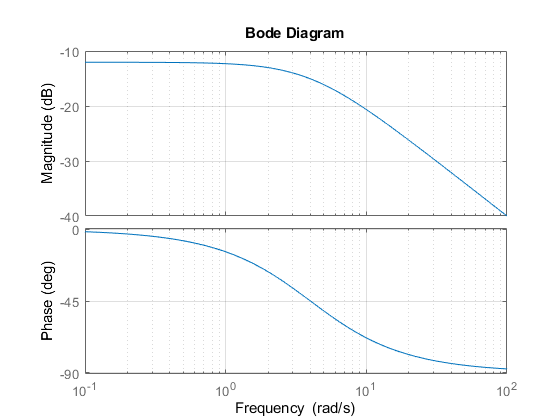
\includegraphics[width=\textwidth]{Bode1Polo}
    \caption{Singolo Polo}
\end{figure}

Si considera un trinomio $\displaystyle\frac{s^2}{\omega_n^2}+\frac{2\xi s}{\omega_n}+1\to_{s=j\omega}-\frac{\omega^2}{\omega_n^2}+\frac{2\xi\omega}{\omega_n}j+1$. 
Per $\omega>>\omega_n$ il modulo sarà: 
\begin{gather}
    \left|-\frac{\omega^2}{\omega_n^2}+\frac{2\xi\omega}{\omega_n}j+1\right|=20\log{10}\left(\sqrt{\left(1-\displaystyle\frac{\omega^2}{\omega_n}^2\right)^2+\frac{4\xi^2\omega^2}{\omega_n^2}}\right)\\
    10\log_{10}=\left(4\xi^2\displaystyle\frac{\omega^2}{\omega_n^2}+\frac{\omega^4}{\omega_n^4}\right)\approx40\log_{10}\left(\displaystyle\frac{\omega}{\omega_n}\right)
\end{gather}
Per $\omega<<\omega_n$ il modulo sarà nullo, poiché: 
\begin{equation}
    20\log{10}\left(\sqrt{\left(1-\displaystyle\frac{\omega^2}{\omega_n}^2\right)^2+\frac{4\xi^2\omega^2}{\omega_n^2}}\right)\approx201log_{10}(1)=0
\end{equation}
Per $\omega=\omega_n$, il modulo dipenderà dallo smorzamento dei poli:
\begin{gather}
    20\log{10}\left(\sqrt{\left(1-\displaystyle\frac{\omega^2}{\omega_n}^2\right)^2+\frac{4\xi^2\omega^2}{\omega_n^2}}\right)=20\log_{10}(2\xi),\:\xi\in[0,1]\\
    20\log_{10}(2\xi)\in(-\infty,20\log_{10}(2)]
\end{gather}
Per uno smorzamento nullo sarà presenta un asintoto verticale per un valore di $\omega=\omega_n$, se non fosse uguale, allora il diagramma di Bode del modulo presenterebbe 
un affossamento nell'intorno di $\omega_n$, la cui profondità aumenta all'aumentare dello smorzamento. Questo affossamento è ciò che causa per i poli il fenomeno della 
risonanza, dove per una certa pulsazione si avrà un guadagno maggiore del guadagno statico del sistema. Per gli zeri si verifica il fenomeno dell'antirisonanza, dove 
per una certa pulsazione risulta estremamente attenuata. La sovraelongazione è un effetto dello smorzamento e sarà massima per smorzamento massimo. \\
Viene definito modulo alla risonanza $M_r$ la distanza tra il picco di risonanza ed il guadadno statico del sistema. 

\begin{center}
    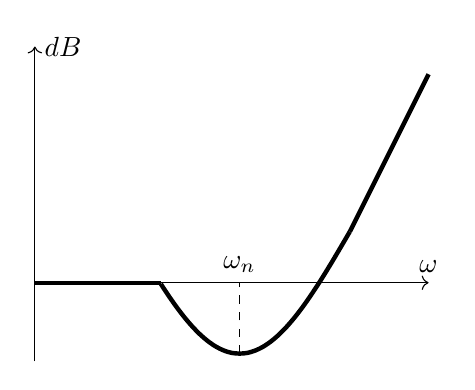
\begin{tikzpicture}[scale=2]
        \draw[->](-1,0)--(1.5,0)node[above]{$\omega$};
        \draw[->](-1,-0.5)--(-1,1.5)node[right]{$dB$};
        \draw[-,ultra thick](-1,0)--(-0.2,0);
        \draw[-, ultra thick]plot[smooth, domain=-0.2:1](\x,{1.55-2*e^-(\x-0.3)^2});
        \draw[dashed](0.3,-0.45)--(0.3,0)node[above]{$\omega_n$};
        \draw[-,ultra thick](1,0.324)--(1.5,1.324);
    \end{tikzpicture}
\end{center}

Per $\omega=0$, a fase del trinomio sarà: $\phase{(1)}=0^{\circ}$, mentre per $\omega\to\infty$, si avrà una fase tendente asintoticamente a: 

\begin{equation}
    \phase{\left(-\displaystyle\frac{\omega^2}{\omega_n^2}+2\xi\frac{\omega}{\omega_n}j+1\right)}\to\phase{-\displaystyle\frac{\omega^2}{\omega_n^2}}=-180^{\circ}
\end{equation}
Mentre per $\omega=\omega_n$, la fase sarà: 
\begin{equation}
    \phase{2\xi j}=90^{\circ}
\end{equation}
Quindi avverrà un cambiamento di fase nell'intorno di $\omega_n$, il cambiamento sarà sempre più rapido per smorzamenti sempre più piccoli, fino a presentare una 
discontinuità per smorzamenti nulli. Per smorzamenti sempre più piccoli la curva nel diagramma di Bode apparirà sempre più schiacciata. \\
Nei sistemi causali ci saranno sempre più poli che zeri, per cui i loro diagrammi di Bode tenderanno sempre a scendere. 

\begin{figure}
    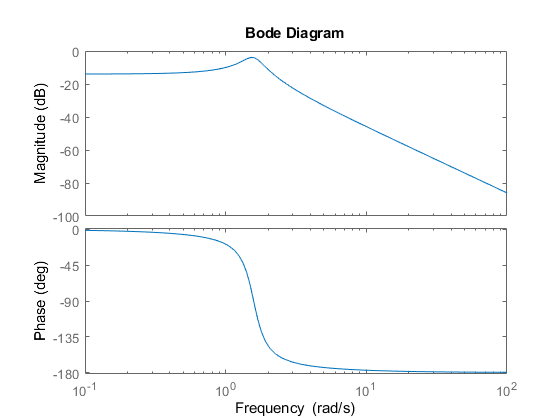
\includegraphics{BodeRisonanza}
    \caption{Fenomeno della Risonanza}
\end{figure}

\subsection{Diagramma di Nyquist}
Data una funzione di trasferimento $M(s)=\displaystyle\frac{s-a}{s-b}$. Si definisce una qualsiasi curva chiusa $\mathbf{G}$ sul piano, e un punto $s$ che percorre la curva in senso 
orario. Allora per uno spostamento di $s$, comporterà uno spostamento di $M(s)$ nel piano di Gauss. 

\begin{center}
    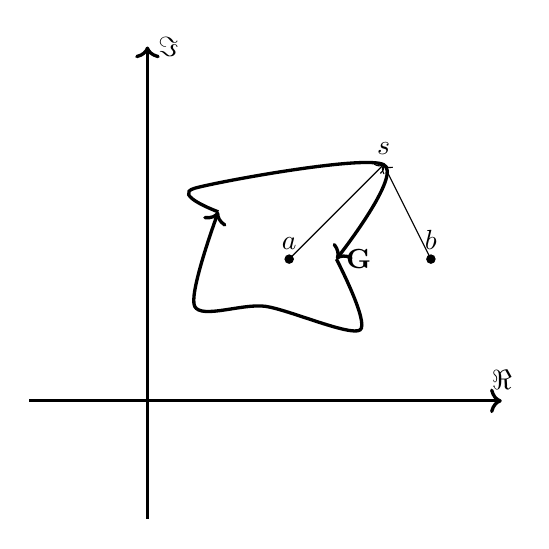
\begin{tikzpicture}[scale=3]
        \draw[->,very thick](0,-0.5)--(0,1.5)node[right]{$\Im$};
        \draw[->,very thick](-0.5,0)--(1.5,0)node[above]{$\Re$};

        \draw[->,very thick]plot[smooth]coordinates{(0.3,0.8) (0.2,0.9) (1,1) (0.8,0.6)};
        \draw[->,very thick]plot[smooth]coordinates{(0.8,0.6) (0.9,0.3) (0.5,0.4) (0.2,0.4)(0.3,0.8)};

        \node[right]at(0.8,0.6){$\mathbf{G}$};

        \node[above]at(1,1){$s$};
        \node[above]at(0.6,0.6){$a$};
        \filldraw[black](0.6,0.6)circle(0.5pt);
        \node[above]at(1.2,0.6){$b$};
        \filldraw[black](1.2,0.6)circle(0.5pt);
        
        \draw[->](0.6,0.6)--(1,1);
        \draw[->](1.2,0.6)--(1,1);
    \end{tikzpicture}
\end{center}

Per determinare se lo spostamento effettuato da $M(s)$ nel piano di Gauss a seguito di una variazione di $s$ formi una curva chiusa, si analizza il cambiamento di 
fase $\phase{M(s)}$. Se il cambiamento di fase della funzione rispetto ad $s$ è nullo allora la curva non ruota attorno all'origine, è un multiplo di $2\pi$: $2k\pi$ 
allora la curva ha ruotato $k$ volte attorno all'origine. Per determinare il cambiamento di fase: 

\begin{equation}
    \phase({M(s)})=\phase{s-a}-\phase{s-b}\\
\end{equation}

Poiché $s$ ruota attorno allo zero $a$, mentre non ruota attorno al polo $b$, il cambiamento di fase $\phase{s-a}$ risulta essere uguale ad una rotazione completa, ovvero 
$2\pi$, mentre $\phase{s-b}=0$ poiché la curva non ruota attorno a $b$. In base alla fase di $\vec{as}$ e $\vec{bs}$ si può ottenere il cambiamento di fase della funzione 
di trasfermento iniziale. Se un punto $s$ ruota intorno ad uno zero od un polo, la fase del vettore distanza $\vec{\alpha s}$ aumenterà fino a $k$-volte le rotazioni 
attorno a quello zero o polo. Si avrà quindi in questo caso:

\begin{equation}
    \phase{M(s)}=2\pi+0
\end{equation}

Quindi la funzione $M(s)$ ruoterà attorno all'origine. 

\begin{center}
    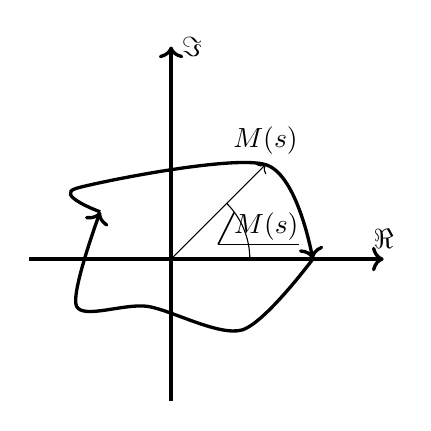
\begin{tikzpicture}[scale=3]
        \draw[->, very thick](0,0.6)--(1.5,0.6)coordinate(x)node[above]{$\Re$};
        \draw[->, very thick](0.6,0)--(0.6,1.5)node[right]{$\Im$};

        \draw[->,very thick]plot[smooth]coordinates{(0.3,0.8) (0.2,0.9) (1,1) (1.2,0.6)};
        \draw[->,very thick]plot[smooth]coordinates{(1.2,0.6) (0.9,0.3) (0.5,0.4) (0.2,0.4)(0.3,0.8)};

        \draw[->](0.6,0.6)coordinate(O)--(1,1)coordinate(M)node[above]{$M(s)$};
        \pic["$\phase{M(s)}$",draw, angle eccentricity=1.2, angle radius=1cm]{angle=x--O--M};
    \end{tikzpicture}
\end{center}

Gli unici termini che contribuiscono al cambiamneto di fase di $M(s)$ sono gli elementi interni alla curva. Poiché il cambiamneto di fase sarà sempre un numero intero di 
rotazioni complete intorno all'origine del piano di Gauss. Si definisce l'indicatore logaritimico $R_{M,0}$, che rappresenta il numero di queste rotazioni. Risulterà 
essere dato da:

\begin{equation}
    R_{M,0}=\#zeri_{\in \mathbf{G}}[M(s)]-\#poli_{\in \mathbf{G}}[M(s)]
\end{equation}

Tramite questo indicatore è possibile determinare graficamente la differenza poli-zeri di una qualsiasi funzione di trasfermineto in $s$. 

Dato un sistema controreazionato, avente una funzione a ciclo aperto $F(s)$, ed una funzione a ciclo chiuso 
$W(s)=\displaystyle\frac{F(s)}{1+F(s)}=1+\frac{N(s)}{D(s)}=\frac{D(s)+N(s)}{D(s)}$. 

\begin{center}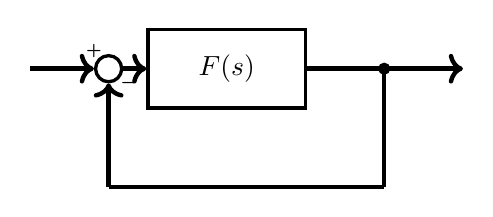
\begin{tikzpicture}[scale=2]
    \node[sum](sum)at(-1,0){};
    \draw[->,ultra thick](-1.5,0)--(sum.180)node[above]{$\scriptscriptstyle\boldsymbol{+}$};

    \node[block, right of=sum, node distance=1.5cm](g){$F(s)$};

    \draw[->,ultra thick](sum.0)--(g.180);
    \draw[-,ultra thick](g.0)--(0.75,0);
    \filldraw[black](0.75,0)circle(1pt);

    \draw[->,ultra thick](0.75,0)--(1.25,0);
    \draw[-,ultra thick](0.75,-0.75)--(0.75,0);
    \draw[-,ultra thick](0.75,-0.75)--(-1,-0.75);

    \draw[->,ultra thick](-1,-0.75)--(sum.270)node[right]{$\scriptscriptstyle\boldsymbol{-}$};
\end{tikzpicture}\end{center}

I poli della funzione a ciclo chiuso corrispodono ai poli di $F$. \\
Applicando il teoroma dell'indicatore logaritimico su $1+F(s)$, si traccia il percorso di Nyquist, una curva chiusa che contiene tutti gli oggetti aventi parte reale 
positiva. La curva si trova interamente sull'asse immaginario, la chiusura avviene all'infinito, per cui la risposta armonica corrisponde al percorso di Nyquist. 

\begin{center}
    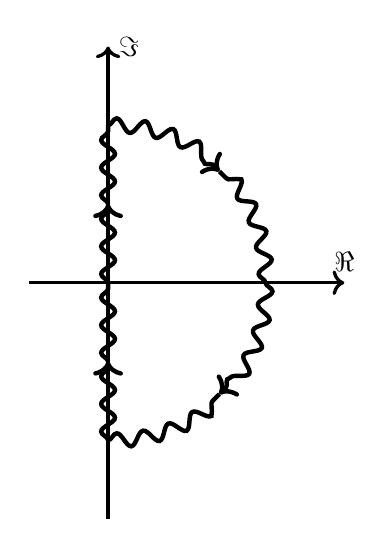
\begin{tikzpicture}[scale=2]
        \draw[->,very thick](-0.5,0)--(1.5,0)node[above]{$\Re$};
        \draw[->,very thick](0,-1.5)--(0,1.5)node[right]{$\Im$};

        \draw[->,snake it, ultra thick](0,-1)--(0,-0.5);
        \draw[-,snake it, ultra thick](0,-0.5)--(0,-0);
        \draw[->,snake it, ultra thick](0,0)--(0,0.5);
        \draw[-,snake it, ultra thick](0,0.5)--(0,1);
        
        \draw[->, snake it, ultra thick](0,1)arc(90:45:1cm);
        \draw[-, snake it, ultra thick](1,0)arc(0:45:1cm);       
        \draw[->, snake it, ultra thick](1,0)arc(0:-45:1cm);
        \draw[-, snake it, ultra thick](0,-1)arc(-90:-45:1cm);

    \end{tikzpicture}
\end{center}

Per cui si ha: 

\begin{equation}
    R_{1+F,0}=\#zeri_{Nyq}[1+F(s)]-\#poli_{Nyq}[1+F(s)]
\end{equation}

Dato che $1+F(s)=\displaystyle\frac{N(s)+D(s)}{D(s)}$, e la funione a ciclo chiuso $W(s)=\displaystyle\frac{N(s)}{D(s)+N(s)}$, gli zeri della funzione $1+F(s)$ equivalgono ai 
poli della funzione a ciclo chiuso, e i poli della funzione $1+F(s)$ equivalgono agli zeri della funzione a ciclo aperto $F(s)$, per cui la differenza poli zeri è data da: 

\begin{equation}
    R_{1+F,0}=\#poli_{Nyq}[W(s)]-\#poli_{Nyq}[F(s)]
\end{equation}

Un sistema è stabile se tutti i poli della sua funzione di trasferimento hanno parte reale positiva, per se il sistema è stabile il numero di poli a parte reale positiva 
sarà nullo: $\#poli_{Nyq}[W(s)]=0$, allora il numero di rotazioni attorno al punto zero di $W(s)$ sarà dato dal solo numero dei poli di $1+F(s)$. Questa relazione è 
reciproca per cui si ha che:

\begin{equation}
    \#poli_{Nyq}[W(s)]=0:\mbox{ sistema stabile}\iff R_{1+F(s),0}=-\#poli_{Nyq}[1+F(s)]
\end{equation}

Traslando la curva di Nyquist di $-1$, si ottiene la risposta armonica della funzione a ciclo aperto $F(s)$. L'indicatore logaritmico di $1+F(s)$ attorno a $0$, quindi 
corrisponde all'indicatore logaritimico di $F(s)$ attorno a $-1$:

\begin{equation}
    R_{F(s),-1}=R_{1+F(s),0}=-\#poli_{Nyq}[F(s)]
\end{equation}

Tramite questa relazione è possibile analizzare il sistema molto più facilmente, poiché la funzione a ciclo aperto è più facilmente alterabile. Se la funzione a ciclo aperto 
è asintoticamente stabile, allora la funzione affinché la funzione a ciclo chiuso stia anch'essa stabile, è necessario e sufficiente che il grafico di $F(s)$ non ruoti 
intorno a $-1$. Questo grafico corrisponde alla risposta armonica della funzione $F(s)$, e viene definito diagramma di Nyquist. A partire dai dati sulla risposta armonica 
forniti dal diagramma di Bode è possibile realizzare il diagramma polare di Nyquist di $F(s)$.  \\

Poiché su un diagramma di Bode vengono rappresentati solo incrementi positivi di $\omega$, si ottiene solo una metà del diagramma di Nyquist. Considerando frequenze negative, 
il modulo poiché deriva da un quadrato rimarrà invariato, mentre la fase sarà opposta. Per cui per il diagramma di Nyquist è simmetrico rispetto alla retta delle ascisse.\\

Se la fase di una funzione di trasferimento non scende al di sotto dei $-180^{\circ}$ allora non potrà mai girare intorno al punto $-1$, poiché il modulo tende sempre 
a $0$ per ogni funzione di trasferimento stabile, per $\omega\to\infty$ il diagramma tende asintoticamente verso l'origine. Il sistema sarà quindi stabile per ogni 
controllore proporzionale maggiore di zero, se invece si sceglie un $Kc$ minore di zero, il sistema sarà stabile fino a quando il diagramma di Nyquist non include il 
punto $-1$. Aumentando il guadagno il diagramma si espande o si comprime, mentre la fase rimane costante, per cui esiste un intrvallo di guadagni negativi per cui il 
diagramma non si espanda oltre il punto $-1$, di conseguenza il sistema è stabile in quell'intervallo. 

\begin{center}
    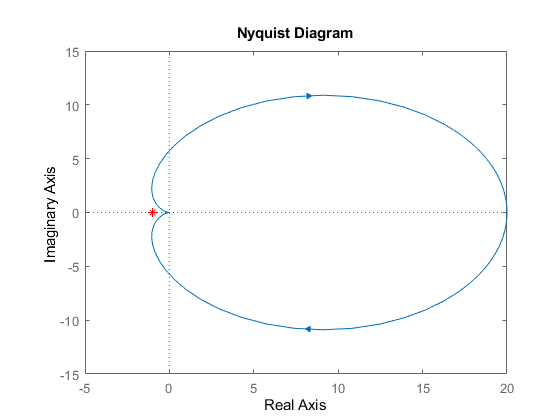
\includegraphics[width=6cm]{Nyquist2.png}
    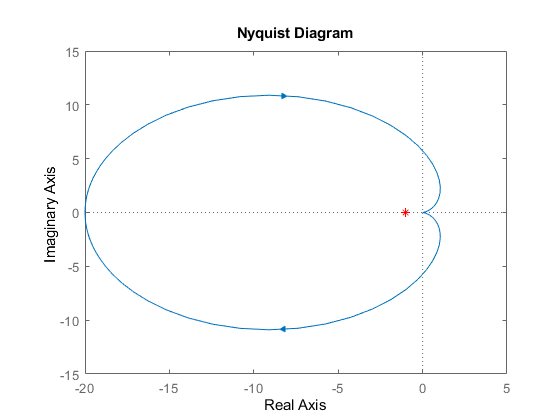
\includegraphics[width=6cm]{Nyquist1.png}
\end{center}

In caso la curva di Nyquist passi sopra un ad un polo, allora si considera un percorso uncinato in modo che $s$ gira intorno al polo $p$, questa rotazione attorno al polo 
causa una variazione di fase aggiuntiva di $180^{\circ}$. 

\begin{center}
    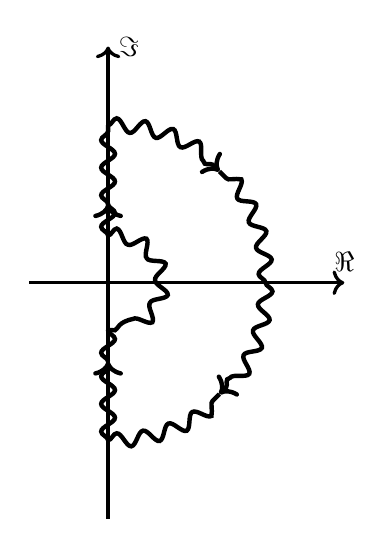
\begin{tikzpicture}[scale=2]
        \draw[->,very thick](-0.5,0)--(1.5,0)node[above]{$\Re$};
        \draw[->,very thick](0,-1.5)--(0,1.5)node[right]{$\Im$};

        \draw[->,snake it, ultra thick](0,-1)--(0,-0.5);
        \draw[-,snake it, ultra thick](0,-0.5)--(0,-0.3);
        \draw[->,snake it, ultra thick](0,0.3)--(0,0.5);
        \draw[-,snake it, ultra thick](0,0.5)--(0,1);

        \draw[-,snake it,ultra thick](0,0.3)arc(90:-90:0.3cm);
        
        \draw[->, snake it, ultra thick](0,1)arc(90:45:1cm);
        \draw[-, snake it, ultra thick](1,0)arc(0:45:1cm);       
        \draw[->, snake it, ultra thick](1,0)arc(0:-45:1cm);
        \draw[-, snake it, ultra thick](0,-1)arc(-90:-45:1cm);

    \end{tikzpicture}
\end{center}



\subsection{Margini di Stabilità}

\subsection{Sistemi con Ritardo}

\subsection{Sistemi a Fase Non Minima}

\subsection{Sintesi Diretta}

\subsection{Stabilità Interna}

\subsection{Guadagno}

\subsubsection{Sensibilità}

\subsubsection{Amplificatori Operazionali}

\subsection{Carta di Nichols}

\subsection{Reti Corretrici}

\subsection{Linearizzazione}

\clearpage

\section{Controllori Digitali}

\end{document}